\documentclass[a4paper]{report}
\usepackage[utf8]{inputenc}
\usepackage[ngerman]{babel}
\usepackage[backend=biber,style=ieee]{biblatex}
\usepackage{graphicx}
\usepackage{xcolor}
\usepackage{setspace} % https://tex.stackexchange.com/questions/83855/change-line-spacing-inside-the-document
\usepackage[paper=a4paper,margin=2.5cm]{geometry}
\usepackage{lmodern} 
\usepackage{fancyhdr} % de.wikibooks.org/wiki/LaTeX-W%C3%B6rterbuch:_fancyhdr
\usepackage{multicol} % overleaf.com/learn/latex/Multiple_columns
\usepackage{amsmath}
\usepackage{lipsum}
\usepackage{dashrule}
\usepackage[toc,page]{appendix}

\renewcommand\familydefault{\sfdefault} % namsu.de/Extra/pakete/Lmodern.html
\definecolor{litec-blue}{HTML}{00305C}

\pagestyle{fancy}                                             % Eigener Seitenstil
\fancypagestyle{plain}{}
\fancyhf{}                                                    % Alle Kopf- und Fußzeilenfelder bereinigen
% \fancyhead[L]{}                                             % Kopfzeile links
% \fancyhead[C]{}                                             % Zentrierte Kopfzeile
% \fancyhead[R]{}                                             % Kopfzeile rechts
\renewcommand{\headrulewidth}{0pt}                            % Obere Trennlinie
\fancyfoot[R]{\textbf{Seite \thepage}}                        % Seitennummer
\fancyfoot[L]{
\includegraphics[scale=0.2]{assets/litec-logo.png}}
% \fancyfoot[C]{\tiny{Typeset with \TeX}}
\renewcommand{\footrulewidth}{0.4pt}                          % Untere Trennlinie

% common references
\addbibresource{references.bib}
% stundent-specific references
\addbibresource{MJ/references.bib}
\addbibresource{GP/references.bib}
\addbibresource{ZB/references.bib}

\begin{document}


\newgeometry{top=2cm,bottom=1cm}

\begin{titlepage}

\begin{center}

% \vspace*{-2cm}

\includegraphics[scale=0.95]{assets/litec-logo-center.png}

\vspace{0.5cm}

{
\Large
\begin{spacing}{1.5}
Höhere Technische Bundeslehranstalt\\
Höhere Lehranstalt für$\ldots$ \textit{Text siehe übernächste Seite}\\
Ausbildungsschwerpunkt$\ldots$ \textit{Text siehe übernächste Seite}
\end{spacing}
}

\vspace{1cm}

{
\Huge
\color{litec-blue}
\textbf{\textit{HTL Diplomarbeit}}
}

\vspace{1.2cm}

{
\Huge
\textit{Diplomarbeitsthema-Thema einfügen}
}

\vspace{1cm}

\begin{spacing}{3}
\textbf{ausgeführt im}\\
{
\Huge
\color{litec-blue}
Schuljahr 20xx/xx
}\\
\textbf{eingereicht von}
\end{spacing}

\vspace{-0.5cm}

\begin{spacing}{1.5}
\hfill
\begin{minipage}{\dimexpr\textwidth-5cm}
\Large
\begin{tabular}{l@{\hskip 4cm}l}
Name & Klasse \\
Name & Klasse \\
Name & Klasse
\end{tabular}
\xdef\tpd{\the\prevdepth}
\end{minipage}
\end{spacing}
\prevdepth\tpd

\end{center}

\vspace{1cm}
\noindent
\Large
Betreuungslehrkraft$\ldots$

\begin{center}
\vfill

\includegraphics[scale=0.15]{assets/htl-bildung-mit-zukunft-logo.jpg}
\end{center}


\end{titlepage}

\newgeometry{margin=2.5cm}
\addtocounter{page}{1}

{
\renewcommand{\thesection}{\Roman{section}.} 
\renewcommand{\thesubsection}{\thesection.\Roman{subsection}}
% https://stackoverflow.com/questions/56301839/signature-page-in-latex
\newcommand\signature[1]{% Name
\begin{center}\begin{minipage}{10cm}
    \centering
    \vspace{3cm}\par
    \noindent
    \hspace{1.5cm}\rule{10cm}{0.5pt}\par
    \noindent
    \hspace{3cm}\textbf{#1}
\end{minipage}\end{center}}

\section{Sperrvermerk}
\lipsum[1]

\vspace{2cm}

\section{Haftungsausschluss}
\lipsum[1]

\newpage

\section{Eidesstattliche Erklärung}
\lipsum[1]

\vspace{2cm}
\noindent
\textbf{Linz, im Juni 20xx}

\signature{\titlePageFullNameGp}
\signature{\titlePageFullNameMj}
\signature{\titlePageFullNameZb}

\newpage

\section{Danksagung}
\lipsum[1]

\newpage

\section{Einleitung}
Dokument wurde mit \LaTeX{} gesetzt.

\newpage

\section{Abstract}
\noindent
\lipsum[10]

}

\newpage
\tableofcontents
\newpage

% chapters
\chapter{Ausgangssituation}
Siehe \cite{LitecHome}

\section{Problemstellung}
\section{Event.kurze Vorstellung des Auftraggebers}
\section{Vorstellung des Projektteam}
\section{Arbeitsaufteilung}
\chapter{Anforderungen an das Projekt}
\section{Grafische Darstellung des Gesamtsystems}
\subsection{Schnittstellen}
\subsection{Komponenten}

\section{Darstellung der Funktionalität mit UML Use Case Diagram}

\section{Zielsetzung}
\subsection{Mussziele}
\subsection{Kann-Ziele}
\subsection{Nicht-Ziel}

\section{Projektplanung}
\subsection{Meilensteine}
\section{Go}\label{sec:tech:go}
Go ist eine für Systemprogrammierung (Dienste, Treiber, etc.) ausgelegte Programmiersprache mit kurzer und prägnanter Syntax. Entwickelt wurde die Sprache unteranderem von Robert Griesemer, Rob Pike und Ken Thompson (vgl. \cite{go:wiki}). Go bietet unteranderem automatische Speicherverwaltung, Typsicherheit, Closures, effiziente Nebenläufigkeitsmechanismen (goroutines). Go wird vor allem als serverseitige Programmiersprache für Webanwendungen und Microservices in Verbindung mit Virtualisierungsumgebungen wie Docker  eingesetzt.
\begin{wrapfigure}{r}{0.35\textwidth}
    \centering
    \includesvg[width=0.19\textwidth]{MJ/assets/Go_Logo_Blue.svg}
    \caption{Go Logo (vgl. \cite{GoLogoBlue})}
\end{wrapfigure}
Die Implementierung des Teilbereichs zur zentralen Schnittstelle des Systems (Kapitel \ref{ch-implementation}) des vorliegenden Projektes wurde ausschließlich in Go verfasst. Da Go eine relativ moderne Programmiersprache ist, und demnach weniger damit vertraut sind, werden in den folgenden Absätzen die wichtigsten Konzepte der Sprache anhand von Beispielen erklärt. Da sich speziell die Konzepte zum Thema Nebenläufigkeit in Go, doch sehr stark von beispielsweise Java oder ähnlichen Sprachen unterscheiden, werden diese hier etwas genauer erklärt um essentielle Teile der Implementierung zu verdeutlichen.\bigskip

\noindent
\textbf{Kurz zum Hintergrund:} \textit{Wieso Go? Wieso nicht Java oder Python?}\\
Der Hauptgrund für den Einsatz von Go als Programmiersprache eines beachtlichen Projektes, wie einer Diplomarbeit, war der Lernfaktor. Nach dem Einsatz von Go im Rahmen einiger privater Projekte, war Ich bereits mit der Sprache sowie dessen Eigenheiten vertraut. Die Alleinstellungsmerkmale (Goroutines, Concurrency, Channels) der Sprache und deren Ausführung, sind zum Großteil sehr elegant und clever gelöst. Vor allem der fehlende Overhead, verglichen mit Technologien wie Java, mit denen man ohne IDE und mehreren Frameworks nicht weit kommt, erleichtert den Entwicklungsprozess sehr. Die kompakte Syntax in Kombination mit statischen Typen ist ebenfalls sehr gut gelöst. Die erwähnten Mechanismen wie goroutines in Kombination mit Channels welche auf den ersten Blick mit Threads vergleichbar sind, erlauben es, anders über Probleme zum Thema Nebenläufigkeit nachzudenken und Lösungen zu finden, welche man mit herkömmlichen Technologien möglicherweise nicht erreicht hätte.\\
Zusammenfassend lässt sich sagen, dass die Beliebtheit von Go in Entwicklerkreisen definitiv gerechtfertigt ist.\bigskip 

\noindent
In den folgenden Abschnitten werden kurz die für die Implementierung relevanten Features der Sprache erklärt.
% \subsection{Relevante Features}
\subsection{Strukturen und Sichtbarkeit}
Ein \mono{struct} ist eine Sammlung von Datenfeldern, an welches Methoden angehängt werden können (vgl. \cite{go:spec:structs}). Structs sind vergleichbar mit Klassen in herkömmlichen Programmiersprachen wie Java. An ein solches Struct können Methoden angehängt werden, welche den Zustand der sich im struct befindlichen Datenfelder verändern.\bigskip

\noindent
\newpage
Hier ein Beispiel wie Structs in Kombination mit Methoden eingesetzt werden um Getter und Setter eines User-Objektes abzubilden. 
{\ColorfulCodeDisclaimer}
% \begin{minipage}[c]{\linewidth}
\begin{lstlisting}[style=goMono,caption={Struct in Kombination mit Methoden}]
type User struct {
    id        int    %\color{magenta}(1)%     
    Firstname string  
    Lastname  string 
}

func %\color{magenta}(2)% (u User) GetId() int {
    return u.id
}

func %\color{magenta}(3)% (u *User) SetId(id int) {
    u.id = id
}
\end{lstlisting}
% \end{minipage}
Im obigen Beispiel werden bereits einige Eigenheiten von Go demonstriert.\bigskip

\noindent
Go regelt die Sichtbarkeit von Variablen, Konstanten, Funktionen und Strukturen anders, manche meinen sogar eleganter, als beispielsweise Java. Es wird nicht jedes Element (Variablen, Funktionen, etc.) einzeln mit einem Sichtbarkeitsmodifizierer wie \mono{public} oder \mono{private} ausgestattet, sondern die Schreibweise des jeweiligen Elements wird beachtet. Elemente, welche mit kleinem Anfangsbuchstaben beginnen sind nur innerhalb der jeweiligen Übersetzungseinheit sichtbar (also innerhalb des \frqq{}\mono{package xyz}\flqq{}). Elemente, die mit großem Anfangsbuchstaben beginnen sind öffentlich sichtbar.\bigskip

\noindent
Mit diesem Hintergrundwissen ausgestattet sollte auch sofort ersichtlich sein wieso für das Attribut \mono{\color{magenta}(1)} \mono{id} Getter und Setter definiert werden müssen. Nun zu \mono{\color{magenta}(2)} und \mono{\color{magenta}(3)}. Dies sind Bespiele für Methoden, also Funktionen die an eine Struktur angehängt wurden und auf die inneren Attribute lesend oder schreibend, zugreifen können. In letzterer Aussage liegt auch gleich der Unterschied zwischen den beiden hervorgehobenen Punkten: lesend, technisch korrekt formuliert \textit{Call-By-Value} und schreibend, also \textit{Call-By-Reference}.  

\newpage
\subsubsection{Struct-Tags}
Datenfelder einer Struktur können mit Attributen ausgezeichnet werden, die von Bibliotheken und Frameworks genutzt werden um beispielweise den JSON-Namen eines Attributes zu definieren (vgl. \cite{go:spec:structs}).\\
Hier ein Bespiel wie \frqq{}struct-tags\flqq{} in Go eingesetzt werden um ein Objekt zu serialisieren.
\begin{lstlisting}[style=goRaw,caption={\centering Objekt \textit{User}, welches mit struct-tags annotiert wurde um die JSON-Serialisierung zu konfigurieren.}]
type User struct {
    ID        int     `json:"-"`
    Firstname string  `json:"my_firstname"`
    Lastname  string  `json:"my_lastname"`
    Skills    []Skill `json:"my_skills"`
}
\end{lstlisting}
Das obige Beispiel demonstriert, wie \frqq{}struct-tags\flqq{} also herkömmliche doppelte Hochkommas (\mono{"}) bzw. rückwärts geneigte Hochkommas (\mono{\`{}}) (engl. \textit{backticks}), dazu verwendet werden, Datenfelder im Struct mit Attributen zu versehen, welche in diesem Fall von dem JSON-Parser in der Standardbibliothek (über ein Reflection Interface im \frqq{}\mono{reflect}\flqq{} package) eingelesen werden. Eine mit \frqq{}\mono{json.Marshal}\frqq{} (vgl. \cite{go:pkg:json:marshal}) serialisierte Instanz der obigen Struktur könnte folgendermaßen aussehen:\\
\verb|{"my_firstname": "Max", "my_lastname": "Mustermann", "my_skills": ["mustern"]}|.\\
Wie erwartet werden die konfigurierten Felder richtig benannt, die \frqq{}Skills\frqq{} auch korrekt als JSON-Array serialisiert und das \mono{ID}-Feld wurde ignoriert da es in der Definition mit \verb|json:"-"| annotiert wurde. 

\subsection{Aufzählungen}
Aufzählungen, auch bekannt unter Enumerationen gruppieren ähnliche Attribute. Aufzählungen in Go funktionieren anders als in Java oder vergleichbaren Sprachen. In Go wird \mono{iota} verwendet um fortlaufende Aufzählungen zu generieren. \mono{iota} ist ein Zähler der standardmäßig bei 0 beginnt und nach jedem Element in der Aufzählung um 1 erhöht wird. Dieses Verhalten kann durch verschiedene Ausdrücke konfiguriert werden. Dieser Zähler wird nach jeder Aufzählung wieder auf 0 zurückgesetzt. Folgendes Beispiel, das eine Aufzählung von verschiedenen Automarken definiert, veranschaulicht das beschriebene Konzept.
\begin{lstlisting}[style=goMono,caption={Aufzählung von Automarken},label={lst:tech:go:enum:ex1}]
const (
    Jeep = iota + 1 %\color{magenta}(1)%
    _
    Audi     
    Mercedes
    Volkswagen
    LandRover
)
\end{lstlisting}
Der Vollständigkeit halber befindet sich im Anhang (siehe Abschnitt \ref{sec:apdx:extendedcode}) der vollständige Go-Code, welcher die im obigen Listing angegebene Ausgabe erzeugt.\\
Hier erfolgt nun eine kurze Erklärung, wie der obige Ausschnitt zu verstehen ist. Die mit \mono{\color{magenta}(1)} markierte Zeile im Listing ist die eigentliche Aufzählung. Hier wird \mono{iota}, eine ganzzahlige Konstante, verwendet um den sich innerhalb der Aufzählung \mono{( ... )} befindlichen Namen einen Wert zuzuordnen. Da \mono{\color{magenta}(1)} die einzige Zuweisung ist, wird diese für die restlichen Namen wiederholt. Nun wird \mono{iota} für jedes Auto um 1 erhöht sodass den Autos schlussendlich folgende Konstanten zugewiesen werden: \mono{Jeep}=1, \mono{Audi}=3, \mono{Mercedes}=4, \mono{Volkswagen}=5, \mono{LandRover}=6. Der \mono{\_} Indentifier steht immer für einen Namen der ignoriert wird, darum wird \mono{Audi} auch der Wert 3, statt 2, zugeordnet.

\subsection{Concurrency Patterns in Go}
\begin{tcolorbox}
\centering\textit{%
\frqq{}Do not communicate by sharing memory; instead, share memory by communicating.\flqq \cite{go:proverbs:concurrency} }
\end{tcolorbox}\bigskip
% https://go.dev/blog/codelab-share
\noindent
Concurrency, dt. Gleichzeitigkeit, also Prozesse welche gleichzeitig ausgeführt werden, sollten in Go dem oben genannten Ideal folgen: Kommunikation zwischen gleichzeitig ablaufenden Prozessen mittels Nachrichtenaustausch. Damit ist gemeint, dass Prozesse die gleichzeitig ablaufen (goroutines), sich über eine gemeinsame Schnittstelle (den Channels) austauschen und synchronisieren sollen anstatt eine im Speicher für alle Prozesse zugängliche, gemeinsame Datenstruktur oder Klasse zu bearbeiten.\bigskip

\noindent
Go stellt diese und weitere Bausteine, die auf diesen Konzepten aufbauen, bereits im Sprachkern bzw. in der Standardbibliothek bereit, sodass keine weiteren Frameworks oder Bibliotheken geladen werden müssen und stellt damit sicher, dass diese effizient und korrekt implementiert sind. In den folgenden Abschnitten werden die für die vorliegende Implementierung (siehe Abschnitt \ref{ch-implementation}) benötigten Konzepte anhand von Beispielen vorgestellt und näher erläutert sodass die weiteren, in der Implementierung benötigten Konzepte, einfacher zu verstehen sind.    

\subsubsection{Goroutines}
Go-routinen sind speichereffiziente Threads, die von der Go-Runtime verwaltet werden (vgl. \cite{go:goroutines}). Sobald eine Funktion mit dem Schlüsselwort \mono{go} vorangestellt wird, wird diese von der Runtime als Goroutine vermerkt und im Hintergrund ausgeführt. Im Vergleich zu Threads sind Goroutinen effizienter, sodass viele Goroutinen gleichzeitig laufen können. Der Programmierer muss sich über die Speicherverwaltung keine Gedanken machen, da dies von der Runtime übernommen wird.\\ Im folgenden Listing wird ein einfaches Beispiel dargestellt, das die Funktionsweise von Goroutinen veranschaulicht: 
\begin{lstlisting}[style=goMono,caption={Beispiel Goroutine},label={lst:go:sync:concurrency:ex1}]
func say(s string) {
	for i := 0; i < 5; i++ {
		time.Sleep(100 * time.Millisecond)
		fmt.Println(s)
	}
}

func main() {
	go say("world") %\color{magenta}(1)%
	say("hello")
}
\end{lstlisting}
Die Funktion \frqq{}\mono{say}\frqq{} wird auf zwei verschiedene Arten aufgerufen. Im ersten Aufruf als Goroutine \mono{\color{magenta}(1)} und im zweiten wird diese im Hauptprogramm (in der Haupt- bzw. Main-Goroutine) aufgerufen. Dabei ist anzumerken, dass das Programm beendet wird sobald das Hauptprogramm abgearbeitet wird, also sobald die Funktion \verb|say("hello")| fünf mal die Zeichenkette \frqq{}hello\flqq{} ausgegeben hat, auch wenn \verb|go say("world")| noch nicht fertig ist. Die Ausgabe auf der Konsole hängt davon ab welche Goroutine der Scheduler (das Programm, welches die Ausführung aller Goroutines verwaltet) zuerst ausführt. Folgende Ausgabe könnte auftreten:
\begin{lstlisting}[style=goMono,caption={Beispiel Goroutine},label={lst:go:sync:concurrency:ex1:output}]
hello
world
hello
world
world
hello
world
hello
hello
\end{lstlisting}
Die Goroutine \verb|go say("world")| konnte nicht vollständig beendet werden da das Hauptprogramm \mono{main()} davor bereits beendet wurde. In der Standardbibliothek befindet sich eine Lösung für dieses Problem. Um auf Goroutinen zu warten, welche noch nicht fertig sind, ohne das diese vom Hauptprogramm abrupt beendet werden, bietet Go eine sogenannte \mono{sync.WaitGroup} (vgl. \cite{go:waitgroup}). Dieser Typ befindet sich im \mono{sync} Paket und muss (zusätzlich zu dem Formatierungspaket \mono{fmt} und dem Paket zur Zeitverwaltung \mono{time}) importiert werden. 

\subsubsection{Synchronisation: \mono{sync.WaitGroup}}
Wie im obigen Abschnitt erläutert können WaitGroup's, welche zur Synchronisation dienen, dazu verwendet das in Listing \ref{lst:go:sync:concurrency:ex1:output} ersichtliche Problem zu beheben.\\
Im nachfolgenden Beispiel wird mit Hilfe einer WaitGroup sichergestellt dass die Goroutine \verb|go say("world")| aus Listing \ref{lst:go:sync:concurrency:ex1} vollständig abgearbeitet wird.

\begin{minipage}[c]{\linewidth}
\begin{lstlisting}[style=goMono,caption={Beispiel Goroutine: Synchronisation mittels \mono{sync.WaitGroup}}, label={lst:go:sync:concurrency:ex2}]
package main

import (
    "time"
    "fmt"
    "sync"
)

func main() {
    var wg sync.WaitGroup 

    wg.Add(1) %\color{magenta}(1)%
    go func() {
        say("world")
        wg.Done() %\color{magenta}(2)%
    }()
    
    say("hello")
    
    wg.Wait() %\color{magenta}(3)%
}
\end{lstlisting}
\end{minipage}
Die Funktion \frqq{}\mono{say}\flqq{} aus Listing \ref{lst:go:sync:concurrency:ex1} bleibt unverändert. Nur der Aufruf als Goroutine wird in eine anonyme Funktion die nun als Goroutine ausgeführt wird, verlagert. WaitGroup's haben einen internen Zähler \mono{\color{magenta}(1)}, der für die Anzahl der laufenden Goroutinen verwendet wird. Mit der Methode \mono{wg.Wait()} wird in diesem Fall die Terminierung des Hauptprogramms solange angehalten, bis dieser Zähler 0 ist. Ist dies der Fall gibt \mono{wg.Wait()} die Kontrolle an den Aufrufer zurück und beendet in diesem Fall das Programm. Der Zähler wird mit \mono{\color{magenta}(1)} um N, in diesem Fall um 1, inkrementiert und mit \mono{\color{magenta}(2)} um 1 dekrementiert. Es wird also solange gewartet \mono{\color{magenta}(3)} bis der Zähler von 1, wieder auf 0 gesetzt wird, was nur dann passiert wenn \frqq{}\verb|say("world")|\flqq{} vollständig ausgeführt wurde. Problem gelöst.  
\subsubsection{Channels}
Channels, also Kommunikationskanäle, sind das in Go primär verwendete Konzept um Daten zwischen den oben vorgestellen Goroutinen auszutauschen (vgl. \cite{go:channels}). Daten können mit dem \mono{<-} Operator auf einen Channel gesendet und davon gelesen werden. Folgendes Beispiel (vgl. \cite{go:channels}) veranschaulicht dieses Konzept.
\begin{lstlisting}[style=goMono,caption={Beispiel Channels},label={lst:go:sync:concurrency:ex3}]
package main

import "fmt"

func main() {
    messages := make(chan string) %\color{magenta}(1)%

    go func() { %\color{magenta}(2)%
        messages <- "ping" %\color{magenta}(3)%
    }()

    msg := <-messages %\color{magenta}(4)%
    fmt.Println(msg)
}
\end{lstlisting}
Go stellt die Funktion \mono{make}, die Instanzen von verschiedenen Typen wie Slices (vergleichbar mit Listen, etc.), Maps und eben auch Channels erzeugt, zur Verfügung. In \mono{\color{magenta}(1)} ist ein Beispiel für die Instanziierung eines Channels über welchen Zeichenketten also \mono{string}'s ausgetauscht werden können, angeführt. Der Name \mono{messages} ist nun eine Referenz auf diesen erzeugten Channel, der nun als Kommunikationsmedium für mehrere Goroutinen zur Verfügung steht. Um den Sachverhalt so einfach wie möglich zu halten, handelt es sich in diesem Beispiel aber nur um eine Goroutine. Die in \mono{\color{magenta}(2)} definierte Goroutine wird in Form einer anonymen Funktion definiert und danach sofort aufgerufen. Dieses Designpattern, dass anonyme Funktionen als Goroutinen ausgeführt werden, wird häufig verwendet, da, wie in diesem Beispiel ersichtlich die Goroutine so direkten Zugriff auf den Channel hat. Die Goroutine besteht nur aus einer Anweisung: \textit{sende die Zeichenkette \frqq{}ping\flqq{}} über den Channel \frqq{}messages\flqq{}, sodass diese von anderen Goroutinen gelesen werden kann. Nachrichten werden wie in \mono{\color{magenta}(3)} ersichtlich mit dem \mono{<-} Operator gesendet. In \mono{\color{magenta}(4)} wird mit demselben Operator wieder vom Channel gelesen. Jedoch ist nun der Channelname rechts vom Operator anstatt links, was anzeigt, dass nun vom Channel gelesen wird und das Ergebnis in der Variable \mono{msg} gespeichert wird.\bigskip

\noindent
\paragraph{Wie wird sichergestellt, das zum Zeitpunkt zu dem der Channel \mono{messages} ausgelesen wird \mono{\color{magenta}(4)}, bereits ein Wert vorhanden ist?} Der \mono{messages} Channel ist ein Beispiel für einen \textit{Unbuffered Channel}, also einen ungepufferten Channel. Dies bedeutet, dass Lese- und Schreiboperationen blockieren. Für das konkrete Beispiel bedeutet das, dass die Leseoperation \mono{\color{magenta}(4)}, solange die Ausführung des Programms blockiert, bis die einzige Schreiboperation \mono{\color{magenta}(3)} ausgeführt wurde.  Würde keine Goroutine auf den \mono{messages} Channel schreiben, aber trotzdem davon gelesen werden, würde das Programm zur Laufzeit mit folgendem Fehler abstürzen:\\ \mono{fatal error: all goroutines are asleep - deadlock!}. Wäre \mono{messages} ein \textit{Buffered Channel}, also ein Channel mit einer konstanten Pufferung, würde die obige Leseoperation nicht blockieren, solange der Channel nicht voll (der Puffer ist mit Nachrichten aufgefüllt) ist. Mehr Informationen zu \textit{Unbuffered Channels} finden sich in der offiziellen Dokumentation (vgl. \cite{go:tour:concurrency}).\\ 

\newpage
\subsubsection{Synchronisation: \mono{sync.Mutex}}\label{sec:tech:go:sync:mutex}
In diesem Abschnitt wird ein weiteres für die Implementierung relevantes Konzept vorgestellt. Ein Mutex sperrt den Zugriff auf einen bestimmten Programmabschnitt für gleichzeitig ablaufende Unterprogramme und gibt diesen, nachdem die Arbeit, die sequentiell ausgeführt werden muss, abgeschlossen ist, wieder frei. Ein Anwendungsfall für ein solches Schloss ist der Zugriff auf eine globale Variable, die von mehreren Goroutinen verändert wird. Generell sollte der Einsatz von globalen Variablen, die in parallel ablaufenden Prozessen verändert werden, eher vermieden werden, doch manchmal ist dies unumgänglich. Um diese Schreibzugriffe zu kontrollieren, kann ein solches Schloss eingesetzt werden. Die beiden Operationen eines Schlosses sind die \mono{.Lock()} und \mono{.Unlock()} Methoden. Im folgenden Beispiel wird dies veranschaulicht:

\begin{minipage}[c]{\linewidth}
\begin{lstlisting}[style=goMono,caption={Beispiel \mono{sync.Mutex}},label={lst:go:sync:concurrency:ex4}]
var lock *sync.Mutex = &sync.Mutex{} %\color{magenta}(1)%

func update(numberPtr *int) { %\color{magenta}(2)%
    for {
        lock.Lock() %\color{magenta}(3)%
        *numberPtr = rand.Intn(1000) %\color{magenta}(4)%
        lock.Unlock() %\color{magenta}(5)%
    }
}
func main() {
    var number int
    go update(&number) %\color{magenta}(6)%
    go update(&number)
}
\end{lstlisting}
\end{minipage}
Der Vollständigkeit halber befindet sich im Anhang (siehe Abschnitt \ref{sec:apdx:extendedcode}), der vollständige Go-Code, der den in diesem Abschnitt vorgestellten Sachverhalt abbildet. Hier wurden lediglich die wichtigsten Teile dargestellt um den Abschnitt kurz zu halten. Doch nun zur Erklärung des obigen Beispiels. In \mono{\color{magenta}(1)} wird ein Schloss definiert, sodass dies für die in \mono{\color{magenta}(2)} definierte Funktion, \mono{update}, welche einer Variable eine Zufallszahl \mono{\color{magenta}(4)} zuweist, zugänglich ist. Vor jedem Schreibzugriff, wird die mit der Funktion geteilten Referenz, \mono{numberPtr}, gesperrt \mono{\color{magenta}(3)}. Nach dem Schreibzugriff wird das Schloss wieder geöffnet \mono{\color{magenta}(5)}. Dies hat einen kontrollierten Zugriff auf den geteilten Speicherbereich zur Auswirkung. \textit{Hinweis}: So sollte natürlich nicht programmiert werden. Dieser Sachverhalt könnte viel effizienter über einen gemeinsamen Channel abgebildet werden.    

\newpage
\subsubsection{Synchronisation: \mono{sync.Cond}}
In diesem Abschnitt wird ein weiteres für die Implementierung relevantes Konzept vorgestellt. Dieser Typ dient dazu, die Benachrichtigung von, in Goroutinen stattfindenden Ereignissen zu erleichtern. Damit ist gemeint, dass man mit Hilfe dieses Typen, die Goroutine B, über ein in Goroutine A stattfindendes Ereignis, benachrichtigen kann. Dieser Typ dient hauptsächlich dazu den Code zu verkürzen und Concurrency-Fehler zu vermeiden die nur schwer nachvollziehbar sind, da dieses Ereignis- und Benachrichtigungssystem auch über Channels in Kombination mit Locks 
(Mutex, siehe Abschnitt \ref{sec:tech:go:sync:mutex} \nameref{sec:tech:go:sync:mutex}) gelöst werden kann.\\
Das nachfolgende Beispiel kombiniert die zuvor bereits vorgestellten Konzepte, \mono{sync.WaitGroup} und \mono{sync.Mutex}, um ein einfaches ereignisgesteuertes Begrüßungssystem abzubilden.
\begin{lstlisting}[style=goMono,caption={Kombination aus Concurrency Konzepten: Begrüßungssystem},label={lst:go:sync:concurrency:ex5}]
func main() {
    var wg sync.WaitGroup
    var cond *sync.Cond = sync.NewCond(&sync.Mutex{}) %\mono{\color{magenta}(9)}%
    
    people := []string{"Nick", "Alecia", "Madison", "Victor", "Travis"} %\mono{\color{magenta}(2)}%
    greetings := []string{} %\mono{\color{magenta}(3)}%
    
    wg.Add(1)
    go func() {
        cond.L.Lock()
        for len(greetings) != len(people) { %\mono{\color{magenta}(5)}%
            cond.Wait() %\mono{\color{magenta}(6)}%
        }
        for _, greeting := range greetings { %\mono{\color{magenta}(7)}%
            fmt.Println(greeting) %\mono{\color{magenta}(8)}%
        }
        cond.L.Unlock()
        wg.Done()
    }()
    
    for _, person := range people {
        cond.L.Lock()
        greetings = append(greetings, greet(person)) %\mono{\color{magenta}(1)}%
        cond.L.Unlock()
    }
    cond.Broadcast() %\mono{\color{magenta}(4)}%
    wg.Wait()
}
\end{lstlisting}
Wie oben erwähnt, kombiniert dieses Beispiel einige der bereits vorgestellten Concurrency Konzepte. Dieses Programm setzt ein einfaches Begrüßungssystem um. Zuerst \mono{\color{magenta}(1)} werden die Begrüßungen aus den gegebenen Namen \mono{\color{magenta}(2)} generiert und in einem Go-Slice (vergleichbar mit einer Liste) \mono{\color{magenta}(3)} abgespeichert. Sobald die Begrüßungen generiert sind sollen die Personen begrüßt werden. Die wartende Goroutine wird mit \mono{\color{magenta}(4)} \mono{Broadcast()} aufgeweckt und überprüft erneut ob die Bedingung, dass alle Begrüßungen generiert wurden (die Länge des \mono{greeting} Slice gleich der Länge des \mono{people} Slice ist) wirklich zutrifft \mono{\color{magenta}(5)} (es könnte ja sein, dass die Goroutine vom Scheduler aufgeweckt wurde, ohne dass die Bedingung zutrifft). Wenn nicht, wird weiter gewartet \mono{\color{magenta}(6)}. Ansonsten werden alle Personen begrüßt \mono{\color{magenta}(7)} (auf der Konsole ausgegeben) \mono{\color{magenta}(8)} und der WaitGroup-Zähler wird mit \mono{Done()} \mono{\color{magenta}(9)} um 1 verringert. Die eigentliche \mono{sync.Cond} Deklaration bekommt im Konstruktor ein \mono{sync.Mutex} Lock übergeben, sodass auf die mit den Goroutinen geteilten Datenstrukturen atomar (also zu jedem Zeitpunkt nur 1 Goroutine), zugegriffen werden kann. Das \mono{sync.Cond} Paket stellt ausserdem noch eine \mono{Signal()} Methode bereit, um nur \textit{eine} Goroutine aufzuwecken, anstatt mit \mono{Broadcast()} alle wartenden Goroutinen aufzuwecken. In diesem Beispiel bleibt das aber gleich, da sowieso nur 1 Goroutine auf ein Signal wartet.\\
Wie gehabt befindet sich das vollständig funktionierende Beispiel im Anhang (siehe Abschnitt \ref{sec:apdx:extendedcode}).

% \subsection{Verwaltung von Abhängigkeiten}
% go-get ...

% \subsection{Generator-Anweisungen}
% ...

\newpage
Docker ist ein Werkzeug, um Software, in einer konfigurierbaren und abgeschotteten Umgebung betreiben zu können (vgl. \cite{wiki:docker}). Docker wird gerne in Verbindung mit Go (siehe Abschnitt \ref{sec:tech:go}) eingesetzt, da Go-Anwendungen auf ein einziges, ausführbares Programm kompiliert werden und daher wenige Abhängigkeiten nach aussen haben.  
\section{Docker}\label{sec:tech:docker}
\begin{figure}[h!] % {r}{0.375\textwidth}
    \centering
    \includesvg[width=0.21\textwidth]{MJ/assets/Docker_logo.svg}
    \caption{Docker Logo (vgl. \cite{DockerLogo})}
\end{figure} 
In der nachfolgenden Implementierung wurde Docker verwendet, um das gesamte System zu containerisieren. Docker kümmert sich um alle Abhängigkeiten und stellt diese den Anwendern im zugehörigen Docker-Hub, zur Verfügung. Dies schränkt den Verwaltungsaufwand einer Software erheblich ein.

\section{MySQL}
MySQL ist ein frei verfügbares, relationales Datenbankverwaltungssystem (vgl. \cite{wiki:mysql}). Damit ist gemeint, dass Tabellen ein \textit{Schema} also eine Struktur haben. Tabellen können über Relationen, in Beziehung zueinander stehen. In Beziehung zueinander stehende Tabellen weisen eine Fremdschlüsselbeziehung auf, die durch ein Foreign-Key Contraint definiert wird. Eine solche Fremdschlüssel Einschränkung definiert, anhand welcher Schlüssel die Tabellen miteinander verbunden sind. 
\begin{figure}[h!]
    \centering
    \includesvg[width=0.19\textwidth]{MJ/assets/MySQL_logo.svg}
    \caption{MySQL Logo (vgl. \cite{MySqlLogo})}
\end{figure} 

\newpage
\section{GORM}\label{sec:theory:orm}
\newacronym{orm}{ORM}{Object Relational Mapper}
% GORM ist ein \acrlong{orm}-Framework für Go. Theoretische Informationen zu \acrlong{orm}'s finden sich im Abschnitt \ref{sec:theory:orm} (\nameref{sec:theory:orm}). Nähere Informationen zu der Programmiersprache Go finden sich im Abschnitt \ref{sec:tech:go} (\nameref{sec:tech:go}). Die Integration von GORM findet hauptsächlich anhand von sog. `struct tags' statt. Diese ist grundsätzlich ein Feature welches Go selbst unterstützt und von GORM ausnutzt wird. 
GORM ist ein \acrlong{orm}-Framework für Go. Nähere Informationen zu der Programmiersprache Go finden sich im Abschnitt \ref{sec:tech:go} (\nameref{sec:tech:go}). Die Integration von GORM findet hauptsächlich anhand von sog. \frqq{}struct tags\frqq{} statt. Diese sind grundsätzlich ein Feature, das Go selbst unterstützt und von GORM ausnutzt wird. 
\subsection{Demonstration anhand eines Beispiels}
Im folgenden Abschnitt wird die Funktionalität des oben erläuterten \acrshort{orm}-Frameworks, \textit{GORM}, anhand eines Beispiels dargestellt. Das folgende Beispiel beschränkt sich lediglich auf die Definition einzelner Objekte, welche von GORM in ein lauffähiges (MySQL) Datenbankschema übersetzt werden. Das Beispiel soll einige Features von GORM demonstrieren, die sich auch in ähnlicher Form in der vorliegenden Implementation wieder finden.
\begin{lstlisting}[style=goMono,caption={GORM Demonstration anhand eines konkreten Beispiels},label={lst:tech:gorm:ex1}]
type Office struct {
  OfficeID   uint     `gorm:"primaryKey"`                    
  Department string   `gorm:"default:'IT'"` %\color{magenta}(4)%
  Workers    []Worker `gorm:"foreignKey:SSN"` %\color{magenta}(1)%
}

type Worker struct {
  SSN       uint      `gorm:"primaryKey"`     
  FirstName string    `gorm:"type:varchar(32)"` 
  LastName  string    `gorm:"type:varchar(32)"`
  OfficeID  uint      `gorm:"foreignKey:OfficeID"` %\color{magenta}(2)%
  Office    Office %\color{magenta}(3)%
}
\end{lstlisting}
Das obige Beispiel demonstriert, wie GORM die Struct-Tags (nähere Informationen dazu im Abschnitt \ref{sec:tech:go} \nameref{sec:tech:go}) der einzelnen Datenfelder der Objekte interpretiert, um so das resultierende Datenbankschema zu konfigurieren. 
Die Beziehung zwischen einem Office, das mehrere Arbeiter beinhaltet, \mono{\color{magenta}(1)} wird auch bereits korrekt abgebildet. GORM verwendet dazu die Reflection Schnittstelle, welche die Go-Runtime zur Verfügung stellt und erstellt die 1-N Fremdschlüsselbeziehung zwischen \textit{Office} und \textit{Worker} da es sich bei dem \mono{Workers} Feld im Office um ein Go-Slice, vergleichbar mit einem dynamischen Array bzw. einer \mono{List<Worker>} in Java, handelt. Weiters wird die \mono{foreignKey} Annotation ausgelesen, um GORM mitzuteilen, über welche Spalte die Beziehung zu definieren ist. Damit auch der \textit{Worker} über seine Zugehörigkeit zu einem \textit{Office} Bescheid weiß, wird auch hier \mono{\color{magenta}(2)}, \mono{\color{magenta}(3)} eine Beziehung zum \textit{Office} definiert.\\
Abschließend wird im Beispiel noch die Definition von Default-Constraints demonstriert \mono{\color{magenta}(4)}: \textit{Office}'s gehören standardmäßig zur IT-Abteilung. GORM generiert aus obigem Go-Code folgendes Datenbankmodell.\bigskip
\begin{figure}[h!]
    \centering
    \makebox[\textwidth][c]{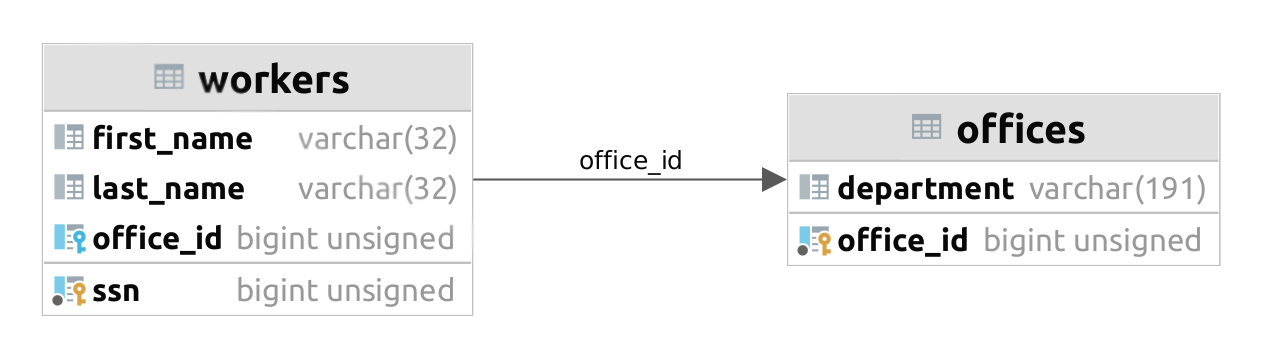
\includegraphics[width=1.15\textwidth]{MJ/assets/schema_office_example_cropped.svg.png}}
    \caption{von GORM aus Listing \ref{lst:tech:gorm:ex1} generiertes Datenbankmodell}
    \label{img:tech:gorm:schema:ex1}
\end{figure}

\newpage
\noindent
In der obigen Abbildung wird auch bereits das Standardverhalten von GORM ersichtlich. GORM hat den Go-Datentyp \mono{string}, der im \mono{Department} nicht genauer definiert wurde als \mono{varchar(191)} übersetzt. Um solche, eher weniger optimalen Abbildungen von Go auf das Datenbankmodell zu vermeiden, sollten Datentypen und Constraints immer explizit definiert werden um Konflikte zu vermeiden. 
Der Vollständigkeit halber befindet sich im Anhang (siehe Abschnitt \ref{sec:apdx:extendedcode}) der komplette Go-Code, der das in Abbildung \ref{img:tech:gorm:schema:ex1} veranschaulichte Datenbankmodell generiert.

\section{Gorilla}\label{sec:tech:gorilla}
Gorilla ist ein für die vorliegende Implementierung zum Einsatz kommendes Go-Toolkit, also eine Sammlung mehrerer Komponenten, mit der schnell und einfach Web Anwendungen entwickelt werden können (vgl. \cite{go:gorilla}). Gorilla beinhaltet Komponenten, unteranderem einen HTTP Multiplexer \mono{gorilla/mux}, der die eingehenden und ausgehenden HTTP-Anfragen an die richtigen Endpunkt-Handler weiterleitet. Eine weitere wichtige Komponente ist die Websocket-Bibliothek \mono{gorilla/websocket}, die ebenfalls für die vorliegende Implementierung zum Einsatz kommt. Schließlich wurde noch die Gorilla-Middleware Bibliothek \mono{gorilla/handlers}, in Kombination mit \textit{Meridian}, dem eigens für dieses Projekt entwickelte Middleware-Framework, eingesetzt.    

% \newpage
% \section{Technologien zur Dokumentation des Projektes}

% % \subsection{Swagger} 
% % (OpenAPI)

% \subsection{Textsatzsystem \LaTeX{}}
% Im Rahmen der vorliegenden Arbeit habe Ich mich umfassend mit dem Textsatzsystem \TeX{} und dessen erfolgreicher Erweiterung, \LaTeX{},  befasst. Auf der Suche nach einem vernünftigen System, um sauber und möglichst effizient, schöne Dokumente zu verfassen, experimentierte Ich mit einigen Systemen wie \textit{groff}, \textit{Markdown} und \textit{Con\TeX{}t}. Markdown zu wenige Features (ohnehin nicht dazu gedacht),  (Ablehnung der Profit und Consumer-orientierten Microsoft Philiosophie sowie zu kompliziert zu Verwenden)\\
% MS Word vs TeX: WYSIWYG vs WYSIWYAF (https://de.wikipedia.org/wiki/WYSIWYG)\\
% dokumentationsprojekt-struktur\\
% verwendete environments um text zu formatieren bzw. grafiken zu generieren\\

\chapter{Theoretische Grundlagen}

\chapter{Theoretische Grundlagen}

\chapter{Theoretische Grundlagen}

\input{MJ/ch4-theoretical-background.tex}
\input{GP/ch4-theoretical-background.tex}
\input{ZB/ch4-theoretical-background.tex}
\chapter{Theoretische Grundlagen}

\input{MJ/ch4-theoretical-background.tex}
\input{GP/ch4-theoretical-background.tex}
\input{ZB/ch4-theoretical-background.tex}
\chapter{Theoretische Grundlagen}

\input{MJ/ch4-theoretical-background.tex}
\input{GP/ch4-theoretical-background.tex}
\input{ZB/ch4-theoretical-background.tex}
\chapter{Theoretische Grundlagen}

\chapter{Theoretische Grundlagen}

\input{MJ/ch4-theoretical-background.tex}
\input{GP/ch4-theoretical-background.tex}
\input{ZB/ch4-theoretical-background.tex}
\chapter{Theoretische Grundlagen}

\input{MJ/ch4-theoretical-background.tex}
\input{GP/ch4-theoretical-background.tex}
\input{ZB/ch4-theoretical-background.tex}
\chapter{Theoretische Grundlagen}

\input{MJ/ch4-theoretical-background.tex}
\input{GP/ch4-theoretical-background.tex}
\input{ZB/ch4-theoretical-background.tex}
\chapter{Theoretische Grundlagen}

\chapter{Theoretische Grundlagen}

\input{MJ/ch4-theoretical-background.tex}
\input{GP/ch4-theoretical-background.tex}
\input{ZB/ch4-theoretical-background.tex}
\chapter{Theoretische Grundlagen}

\input{MJ/ch4-theoretical-background.tex}
\input{GP/ch4-theoretical-background.tex}
\input{ZB/ch4-theoretical-background.tex}
\chapter{Theoretische Grundlagen}

\input{MJ/ch4-theoretical-background.tex}
\input{GP/ch4-theoretical-background.tex}
\input{ZB/ch4-theoretical-background.tex}
In diesem Kapitel werden die verschiedenen Komponenten des Systems, sowie deren Zusammenspiel erläutert. % Beginnend wird das System in Form eines UML Use-Case Diagramms grafisch dargestellt, welches eine grobe Übersicht vermitteln soll. Danach wird das System in den einzelnen Komponenten genauer erklärt.   

\section{Architektur der zentralen Schnittstelle des Systems}
% \textit{Insert graphical representation of the system here\ldots}
In den nachfolgenden Abschnitten wird die Implementierung der zentralen Schnittstelle des Systems in technischen Details erläutert. In Abbildung \ref{fig:impl:dir-structure} ist die grobe Ordnerstruktur der vorliegenden Implementierung veranschaulicht. Diese einzelnen Komponenten sowie deren Schnittstellen zueinander werden dem Leser im nachfolgenden Kapitel und Abschnitten anhand von Erklärungen, Fallbeispielen, und Grafiken im Detail erläutert. Weiters werden die getroffenen Designentscheidungen jeweils motiviert, sodass auch im Sinne des technischen Entwurfs die Zweckmäßigkeit dahinter ersichtlich ist. Ein Programm, in diesem Fall ein Softwaresystem, sollte vor dessen Einsatz immer und möglichst gründlich getestet werden. \newpage Um das im Zuge dieser Arbeit entstandene System zu testen, reichten einfache Unit-Tests nicht aus. Daher musste das gesamte System zuerst simuliert werden, bevor es getestet werden konnte. Dazu wurden zwei Simulatoren entwickelt, welche einerseits die Kommunikation zwischen Benutzer und Server, also eine übliche Client-Server Architektur und andererseits zwischen Schließfächern und Server, simulieren.
\begin{wrapfigure}[17]{r}{.225\textwidth}
\begin{lstlisting}[style=directoryListing,label={lst:impl:dirstructure}]
.
├── api
│   ├── auth
│   ├── controller
│   ├── docs
│   ├── meridian
│   ├── model
│   ├── observer
│   ├── paths
│   ├── response
│   └── util
├── broker
│   └── volumes
├── persistent
├── sandbox
└── simulator
    ├── client
    └── controller
\end{lstlisting}
\caption{Verzeichnis-Struktur der Implementierung}
\label{fig:impl:dir-structure}
\end{wrapfigure}
Aufgrund der mit Docker unterstützten Containerisierung der zentralen Schnittstelle ist man in Sachen Verzeichnisstruktur teilweise etwas eingeschränkt, wodurch man sich sehr genau überlegen muss, in welche Komponenten und demnach Softwarepakete man das System am besten unterteilt. Mehr Informationen zur Containerisierung des Systems finden sich ebenfalls in diesem Kapitel. Die oben kurz angeschnittenen Simulatoren befinden sich im gleichnamigen \mono{simulator} Verzeichnis. Die \mono{broker}- und \mono{persistent} Verzeichnisse enthalten Konfigurationsskripte sodass die sich im \mono{docker-compose.yml} befindlichen MQTT- und MySQL-Images korrekt konfiguriert werden. In der \mono{sandbox} befanden sich während der Entwicklung Implementierungen von Komponenten auf einem kleineren Maßstab, die später, entweder in das Gesamtsystem, also in das \mono{api} Verzeichnis aufgenommen wurden, oder durch bessere Lösungen ersetzt wurden. Im \mono{api} Verzeichnis befindet sich die eigentliche Implementierung der zentralen Benutzer- und Controller Schnittstelle. Datenbankschemas, die mithilfe von GORM definiert wurden, befinden sich im \mono{model} Verzeichnis. Regeln, für die auf Seiten der Benutzerschnittstelle erforderlichen Authentifizierung, wurden im \mono{auth} Verzeichnis definiert. Die sich im \mono{controller} und \mono{observer} befindlichen Programmbibliotheken bilden die Grundlage für die Schnittstelle zwischen Server und Schließfächern. In der \mono{response} wird die REST Schnittstelle zum Benutzer definiert. Das als \textit{Meridian} getaufte Middleware Framework befindet sich im gleichnamigen Verzeichnis und bildet die Grundlage für die in beiden übergeordneten Schnittstellen zum Einsatz kommende Middleware. Mehr Informationen dazu finden sich in den folgenden Abschnitten. Im \mono{paths} Verzeichnis befinden sich Konstanten, wie API-Endpunktnamen sowie Reguläre Ausdrücke zur Validierung von Benutzerdaten. Im \mono{util} befinden sich etwaige global benötigte Typen- und Funktionsdefinitionen. % In \mono{docs} befindet sich die automatisch generierte Swagger API-Dokumentation welche im Anhang \ref{sec:apdx:api_reference} ersichtlich ist und aus den im Programmcode annotierten Endpunkt-Handlern erzeugt wird.   
Wichtig im Zusammenhang der oben erklärten \textit{Verzeichnisse} zu erwähnen ist, dass dies vielmehr \textit{Go-Module} sind, also von Go mit jeweils einer zugehörigen \mono{go.mod} Konfigurationsdatei erkannte \textit{Pakete}, welche im Programm referenziert werden. 

\section{Datenbankmodell}\label{sec:impl:database}
In diesem Kapitel der Implementierung wird das Datenbankmodell des Systems anhand der Anforderungen an das Projekt näher erläutert. Auf Abbildung \ref{fig:dbschema} (\nameref{fig:dbschema}) findet sich eine grafische Aufbereitung des Datenbankmodells. Zuvor jedoch wird die Motivation hinter dem vorliegenden Modell auf Basis der zu speichernden Daten, nämlich Benutzer, welche sich Karten aus Schließfächern ausborgen bzw. reservieren können, hervorgehoben.\bigskip

\noindent
Die zentrale Tabelle des Modells stellt das \textit{Schließfach} dar. In der im Modell als \mono{storages} abgebildeten Tabelle befinden sich alle Informationen zu einem Schließfach. Ein Schließfach zeichnet sich durch dessen Kapazität, also wieviele Schlüsselkarten darin Platz haben, als auch einem eindeutigen Namen aus, unter dem dieses dem Benutzer bekannt ist. Jedes Schließfach ist genau einem Raum im Gebäude zugeordnet in welchem es sich gerade befindet. Um die Verwaltung der Schließfächer im Netzwerk zu erleichtern besitzt jedes Schließfach außerdem ein Adressfeld worin sich standardmäßig die Schuldomain \textit{schule.local} befindet, welches aber beispielsweise für die Speicherung der IP-Addresse eines sich im Netzwerk befindlichen Schließfaches genutzt werden kann.\bigskip

\noindent
Ein Schließfach beheimatet mehrere \textit{Karten}. Jede Karte zeichnet sich durch einen eindeutigen Namen und einer Position im Schließfach aus. Die auf einer Schlüsselkarte gespeicherten Bytefolge ist ebensfalls Teil einer Karte im Datenbankmodell. Details, wie sichergestellt wird, dass diese Bytefolge korrekt übertragen und in der Datenbank gespeichert wird, finden sich im Abschnitt \ref{sec:centralAPI} (\nameref{sec:centralAPI}). Weiters wird pro Karte die Anzahl der Zugriffe, also wie oft diese bereits in Verwendung war, protokolliert und ob diese derzeit in Verwendung ist.\bigskip

\newpage
\noindent
Karten können reserviert oder ausgeborgt werden. Dieser Prozess wurde in der\\ \mono{reservations} Tabelle abgebildet. Eine Reservierung setzt sich allgemein aus der eindeutigen Kartenidentifikationsnummer sowie der Benutzeridentifikationsnummer, dem Zeitstempel an dem die Karte reserviert wurde, dem Zeitstempel zu dem die Karte \textit{vorraussichtlich} wieder zurückgegeben wird, sowie dem Zeitstempel an dem die Karte \textit{tatsächlich} wieder zurückgegeben wurde, zusammen.    
Wie bereits erwähnt, wird zwischen reservieren und ausborgen von Karten unterschieden. Mit \frqq{}\textit{ausborgen}\flqq{} ist gemeint, dass die Karte, wenn diese derzeit verfügbar ist, dem Schließfach nach dem Anmeldevorgang in der App bzw. am Schließfach Display direkt entnommen wird. Mit \frqq{}\textit{reservieren}\flqq{} ist gemeint, das die Karte für einen zukünftigen Zeitpunkt reserviert wird, sodass davon auszugehen ist, das diese auch für den bestimmten Zeitraum verfügbar sein wird.
Wird eine Karte direkt vom Schließfach entnommen gilt diese als ausgeborgt. Dieser Unterschied wird im Datenbankmodell mit Hilfe des \frqq{}\mono{is\_reservation}\flqq{} Flags abgebildet. In diesem Fall werden auch die zuvor erwähnten Zeitstempel nur teilweise befüllt. Das Rückgabedatum einer Reservierung \frqq{}\mono{until}\flqq{} wird in diesem Fall mit \frqq{}\mono{NULL}\flqq{} befüllt und \frqq{}\mono{is\_reservation}\flqq{} wird auf \frqq{}\mono{0}\flqq{} bzw. \frqq{}\mono{false}\flqq{} gesetzt.\bigskip

\noindent
\newglossaryentry{admin}{name={Administrator}, description={Benutzer, mit erhöhten Berechtigungen im System}}
\textit{Benutzer} gehören zu Reservierungen. Ein Benutzer zeichnet sich durch eine eindeutige E-Mail-Adresse und dessen Schlüsselkartendaten aus. Es gibt Benutzer, sog. \gls{admin}en, welche erhöhte Berechtigungen im System haben. Administratoren sind \frqq{}\mono{privileged}\flqq{}, während dieses Flag bei herkömmlichen Benutzern standardmäßig auf \frqq{}\mono{0}\flqq{} bzw. \frqq{}\mono{false}\flqq{} gesetzt ist. Spezifische Informationen zu Berechtigungen zwischen herkömmlichen Benutzern und Administratoren finden sich im Abschnitt \ref{sec:centralAPI} (\nameref{sec:centralAPI}), genauer \frqq{}\nameref{sec:privilegesAndAuthorization}\flqq{}. Details, wie sichergestellt wird, dass die auf der Schlüsselkarte eines Benutzers gespeicherte Bytefolge (\frqq{}\mono{reader\_data}\flqq{}) korrekt übertragen und in der Datenbank gespeichert wird, finden sich ebenfalls im genannten Abschnitt. 
Die Eindeutigkeit von E-Mail-Adressen, Kartennamen und Schließfachnamen schränkt möglicherweise die Namensvergabe von beispielsweise Karten innerhalb eines Schließfaches ein, jedoch dient es der Nachvollziehbarkeit und vor allem der Einfachheit des Modells. Diese Einschränkung, dass beispielsweise keine Karte denselben Namen haben kann auch wenn diese zu unterschiedlichen Schließfächern gehört, ist der Motivation geschuldet, das Modell so einfach wie möglich zu halten aber dennoch alle Anforderungen abzudecken.\bigskip

\newpage
\noindent
\textbf{Zusammenfassung des Datenbankmodells}:
\begin{description}\setlength\itemsep{1.5em}

\item[\mono{storages}] Hier werden alle Schließfächer gespeichert. Ein Schließfach hat einen eindeutigen Namen sowie einen Raum im Gebäude dem es zugeordnet ist und eine Kapazität, also wieviele Karten darin Platz haben. Zur Verwaltung der Karten im Netzwerk hat ein Schließfach ausserdem ein \frqq{}Adressfeld\flqq{} worin z.B. die IP-Adresse des Schließfach-Controllers gespeichert wird. Weiters hat ein Schließfach eine Fremdschlüsselbeziehung zu denen sich im Schließfach befindlichen Karten.

\item[\mono{cards}] In dieser Tabelle werden alle verfügbaren Karten gespeichert. Eine Karte gehört, anhand dem \mono{storage\_id} Fremdschlüssel zu genau einem Schließfach. Eine Karte kann mehrmals reserviert werden. Dies wird durch den sich in der Reservierungstabelle befindlichen Fremdschlüssel, welcher auf eine Karte zeigt, abgebildet. Eine Karte hat einen eindeutigen Namen, Zugriffszähler, Position im Schließfach, sowie eine textuelle Repräsentation der auf der Karte gespeicherten Bytefolge. Eine Karte ist zu jedem Zeitpunkt entweder \textit{verfügbar} oder \textit{nicht verfügbar}.   

\item[\mono{reservations}] Sobald eine Karte das Schließfach verlässt wird eine \textit{Reservierung} angelegt. Wird eine Karte für einen zukünftigen Zeitpunkt reserviert, so werden die jeweils die Eckdaten der Reservierung protokolliert (siehe genauere Erklärung oben). 

\item[\mono{users}] Benutzer und Administratoren finden sich in der \mono{users} Tabelle. Benutzer und Administratoren unterscheiden sich im Datenbankmodell durch deren \mono{privileged} Feld. Zu einem Benutzer gehört jeweils eine eindeutige E-Mail-Addresse sowie die eindeutigen Kartendaten auf dessen Schlüsselkarte. \textit{Bemerkung}: Die sich derzeit im Einsatz befindlichen \textit{Schlüssel-Chips}, werden ebenfalls als \frqq{}\textit{Schlüsselkarten der Benutzer}\flqq{} bezeichnet.  
\end{description}

\newpage\vfill
\begin{center}    
    \makebox[\textwidth][c]{\includesvg[width=1.15\textwidth,inkscapelatex=false,pretex=\escapeus]{MJ/assets/schema_channel_light_min.svg}}
    \captionof{figure}{Beziehungen der Tabellen im Modell}
    \label{fig:dbschema}
\end{center}
\newpage
\noindent
Das vorliegende Datenbankmodell wurde mit Hilfe eines \acrlong{orm} in die zentrale Schnittstelle des Systems integriert. Ein umfassender theoretischer Hintergrund zum \acrlong{orm} findet sich im Abschnitt \ref{sec:theory:orm} (\nameref{sec:theory:orm}). Kurz zusammengefasst, stellt eine \acrshort{orm}-Bibliothek bzw, Framework, eine Übersetzungsschicht zwischen Programmiersprache und Datenbank dar. Anstatt direkt mit Tabellen, wird mit Objekten gearbeitet, welche von der \acrshort{orm}-Bibliothek verwaltet werden. \bigskip

\noindent
Konkret kam \textit{GORM}, \frqq{}The fantastic ORM library for Golang\flqq{} \cite{gorm},  zum Einsatz. Das Framework stellt eine sehr angenehme und gut durchdachte Schnittstelle zur Datenbank dar. Weiters stellen die GORM-Autoren auch Treiber für viele verschiedene Arten von relationalen Datenbanken zur Verfügung\cite{gorm:drivers}. Für die vorliegende Implementation wurde der MySQL-Treiber für GORM verwendet. Die Umstellung des gesamten Systems auf beispielsweise PostgreSQL wäre jedoch ein leichter, da das Datenbankmodell absolut plattformunabhängig ist und auf allen von GORM unterstützten Datenbanksystemen lauffähig ist. Die vorliegende Implementierung verwendet den GORM-MySQL Treiber in Kombination mit dem offiziellen MySQL Docker-Image (vgl. \cite{mysql:docker-image}). 

\noindent
MySQL wurde als Datenbanksystem ausgewählt da es der de-facto Standard für viele Systeme mit kleinen bis mittelgroßen Anforderungen ist, einfach zu konfigurieren ist, viel Dokumentation vorhanden ist und am wichtigsten, schnell und verlässlich funktioniert. Das offizielle Docker-Image, das vom MySQL-Team bereitgestellt wird, ist ebenfalls sehr einfach zu konfigurieren und wahrscheinlich noch wichtiger, angenehm in ein bereits vorhandenes Docker-Image zu integrieren (was man von einigen Docker-Images nicht behaupten kann, siehe Kompatibilitätsprobleme, Konflikte zwischen Containern, fehlende Dokumentation etc.). Für mehr Informationen zur Konfiguration des Systems im Hinblick auf Docker, siehe Abschnitt \ref{sec:impl:docker} (\nameref{sec:impl:docker}). Die Technologie \frqq{}Docker\flqq{}, wird allgemein im Abschnitt \ref{sec:tech:docker} (\nameref{sec:tech:docker}) näher erläutert. 

\newpage
\section{Zentrale Benutzer-- und Controller--Schnittstelle}\label{sec:centralAPI}
\newglossaryentry{server}{name={Server}, description={Mit \textit{Server} ist, im engeren Sinne der Implementierung des vorliegenden Projektes, die zentrale Schnittstelle zwischen Benutzer und Schließfächer gemeint}}
In den folgenden Abschnitten wird die Implementierung der Zentralen Schnittstelle, welche als Knotenpunkt zwischen den Benutzern der beiden im Rahmen der Diplomarbeit entwickelten App's sowie der Steuerungssoftware der Schließfächer dient, erläutert. Der Aufbau der vorliegenden Implementierung entspricht einer zentralisierten Client-Server Architektur. Dies hat den Vorteil, dass alle zu speichernden Daten von genau einer Einheit im System, dem Server, verwaltet werden. Dies dient einerseits der Konsistenz der Daten in dem Sinne, da der Server zu jedem Zeitpunkt die Berechtigungen des Benutzers überprüft, der auf die Daten zugreifen möchte und demnach auch Anfragen ablehnt, zu denen dem Benutzer die Berechtigungen fehlen. Andererseits sind auch dadurch auch die Clients im Netzwerk unabhängig voneinander, da der Server eine Schnittstelle bereit stellt, welche die Clients abfragen, um so Informationen zu erhalten.\bigskip

% Es wurde unterschieden zwischen Zustandslosen HTTP Abfragen und   
% Die einzelnen Komponenten dieser zentralen Schnittstelle 
\noindent
Die vorliegende Implementierung stellt, wie man wahrscheinlich bereits aus der obigen Überschrift ableiten kann, zwei übergeordnete Schnittstellen zur Manipulation des Systems bereit. Einerseits eine über HTTP erreichbare REST-Schnittstelle (genauere Informationen zur \acrshort{rest}-Architektur finden sich im Abschnitt \ref{sec:theory:rest} \nameref{sec:theory:rest}) und andererseits eine über MQTT (mehr Informationen dazu im Abschnitt \ref{sec:theory:mqtt} \nameref{sec:theory:mqtt}) erreichbare Schnittstelle, die für den Austausch von Daten zwischen den Schließfächern zuständig ist. Diese beiden übergeordneten Schnittstellen setzen sich client-seitig aus HTTP-Endpunkten und auf seiten der Schließfach-Controller aus MQTT-Topics und den dazugehörigen \textit{Aktionen} zusammen. Der \gls{server}, auf dem diese beiden Schnittstellen erreichbar sind, wird in den nachfolgenden Abschnitten sowohl textuell als auch in Form von Grafiken und Programmbeispielen näher erläutert. 

\subsection{Architektur des Servers}
% Eventmodel, "Postamt"
Die Architektur des \gls{server}s lässt sich am besten mit einem Postamt, in dem die Post protokolliert und schlussendlich an den wirklichen Empfänger weitergeleitet wird, vergleichen. Nachdem das Postamt die Post an den Adressaten weitergeleitet hat und dessen Antwort retour angekommen ist, wird der Absender, der die Kommunikation angestoßen hat über die Antwort seines Adressaten informiert. Soweit zum Vergleich der Architektur mit einem Postamt.\bigskip

\noindent
Die primäre Aufgabe des \gls{server}s ist es einerseits \textit{die Post zu protokollieren}, also eine Schnittstelle zur Datenbank zur Verfügung zu stellen um kontrolliert Daten darin zu manipulieren und abzufragen. Andererseits dient der Server auch als Vermittlung zwischen den Clients, also den Professoren und Administratoren, die über die von den Kollegen zur Verfügung gestellten Anwendungen, die Client-Schnittstelle nutzen. Weiters übernimmt der Server die alleinige Kommunikation mit allen verfügbaren Schließfächern in denen die Schlüsselkarten abgelegt sind.\bigskip

\noindent
Die Schnittstelle des Servers zu den beiden entwickelten Apps, stellt den größten Teil der vorliegenden Implementierung dar. Aus diesem Grund wird diese zuerst vorgestellt.

\newacronym{api}{API}{Application Programming Interface, dt. Schnittstelle zu einem System}
\newacronym{rfid}{RFID}{Radio Frequency Identification}
\newglossaryentry{resourceHandler}{
    name=Resource Handler,
    description={Funktion, welche aufgerufen wird, sobald ein Endpunkt der HTTP Schnittstelle aufgerufen wird.}
}
\subsection{Client Schnittstelle}
Server und Client tauschen Informationen jeweils \textit{synchron} als auch \textit{asychron} miteinander aus. Informationen, die der Client vom Server anfordert bzw. dem Server übermittelt werden, werden mithilfe der \acrshort{rest} Schnittstelle synchron übertragen. Damit ist konkret gemeint, dass der Server den im \gls{resourceHandler} für den jeweiligen Endpunkt definierten Ablauf, sequentiell (Schritt für Schritt) abarbeitet und der Client solange auf die Antwort vom Server wartet, bis dieser entweder antwortet oder eine Zeitüberschreitung erfolgt.\\
Informationen, die der Server nicht ohne Unterstützung eines Schließfach-Controllers bereitstellen kann, werden asychron übermittelt.\\
Damit ist allgemein gemeint, dass sobald der Client die Anfrage an den Server gestellt hat, dieser sich anderen Arbeiten widmen kann. Sobald der Server dem Client die Antwort übermittelt hat, wird der Client über die Ankunft der Informationen informiert und interpretiert diese nun innerhalb eines Event-Handlers oder Interrupt-Routine.\\
Konkret findet asynchroner Datenaustausch zwischen Client und Server, in Form von Websockets, immer dann statt, wenn Schließfächer involviert sind. Beispielsweise möchte sich ein Benutzer, die Karte \mono{Card\_3-28\_1}  über den sich am Schließfach befindlichen Touchscreen ausborgen. Die Anwendung, die der Benutzer über den Touchscreen navigiert, sendet eine HTTP-PUT Anfrage an einen Endpunkt der \acrshort{rest} Schnittstelle, konkret\\ \frqq{}\mono{/api/v1/storages/cards/name/Card\_3-28\_1/fetch}\flqq{}.  Die gewünschte Karte wird im \acrshort{uri} übergeben.\bigskip
% mit folgendem JSON-Body (der HTTP-Header wird in diesem Beispiel nicht genauer erläutert: für die Implementierung relevanten Header, werden in nachfolgenden Abschnitten und vorrangig in der angehängten API-Dokumentation näher besprochen):
% \begin{lstlisting}[style=goRaw]
% {}
% \end{lstlisting}

\newpage
Diese vom Benutzer geforderte Aktion muss schrittweise abgearbeitet werden:
\begin{enumerate}[label=\textbf{Schritt (\roman*)}]\setlength\itemsep{1.5em}
\item Der Server überprüft ob der Benutzer authentifiziert und dazu berechtigt ist diesen Endpunkt zu verwenden. 
\item Der Server überprüft ob die vom Benutzer angeforderte Karte existiert.
\item  Sofern die Karte existiert, wird in der Datenbank überprüft ob diese gerade in Verwendung ist: \mono{cards.is\_available == 1}
\item Sofern die Karte gerade verfügbar ist, sendet der Server nun eine Nachricht per MQTT an das Schließfach, genauer an den Schließfach-Controller, in dem sich die Karte befindet und bittet den Benutzer, seine Schlüsselkarte an dem sich am Schließfach befindlichen \acrshort{rfid} Leser, zu scannen. (Genau 
genommen sendet der Server eine \textit{Action} an das Topic des Schließfach-Controllers: mehr dazu in Abschnitt \ref{sec:impl:storagecontroller} \nameref{sec:impl:storagecontroller}) 
\item Ist der Benutzer bereits mit seiner E-Mail-Adresse und Kartendaten registiert, ist dieser berechtigt sich die Karte vom Schließfach auszuborgen, andernfalls muss sich dieser erst registrieren und den Ausleihe-Vorgang neu starten. Sofern der Benutzer registriert ist, sendet der Server nun eine Bestätigung an den Schließfach-Controller sodass dieser die Karte freigibt.
\item Der Schließfach-Controller sendet eine Bestätigung über den Erfolg oder Fehler der Aktion an den Server zurück.
\item Der Server erhält diese Bestätigung und wertet aus ob diese erfolgreich war, also\\ \verb|{ ... "successful": true ... }|. Sofern diese erfolgreich war, schreibt der Server die Änderungen in die Datenbank. In beiden Fällen informiert der Server die Teilnehmer des Websockets über die Resultate der Transaktion.
\end{enumerate}

\subsubsection{Endpunkte der Benutzer-Schnittstelle}
Die Benutzer-Schnittstelle ist im Anhang \ref{sec:apdx:api_reference} umfassend dokumentiert. Dort werden alle Endpunkte samt deren HTTP-Methoden, Headern, Authentifizierung und mindestens benötigten Rechten dokumentiert. In diesem Abschnitt wird lediglich der Aufbau und die Struktur der REST-API-Endpunkte näher erläutert.\bigskip

\noindent
Die Benutzer-Schnittstelle stellt Endpunkte für folgende Kategorien zur Verfügung:
\begin{description}
\item[Schließfächer \mono{/api/v1/storages/*}] Die Benutzer-Schnittstelle stellt Endpunkte zum Erstellen, Ändern, Löschen und gefilterten Abfragen von Schließfächern bereit. Nachdem Schließfächer erstellt wurden, sind diese noch nicht einsatzbereit. Damit ist gemeint, dass der Server noch nicht deren MQTT Topic folgt (subscribe). Dadurch können mehrere Schließfächer erstellt werden ohne dass diese gerade erreichbar sein müssen. Um den Server auf einen erreichbaren Schließfach-Controller zu \textit{fokussieren} stellt die Benutzer-Schnittstelle einen entsprechenden Endpunkt zur Verfügung.
\item[Karten \mono{/api/v1/storages/cards/*}] Die Benutzer-Schnittstelle stellt Endpunkte zum Erstellen, Ändern, Löschen und gefilterten Abfragen von Karten bereit. Karten können entweder von einem Benutzer, der die mobile Anwendung verwendet, ausgeborgt bzw. reserviert werden oder von einem Benutzer, der das Display am Schließfach bedient, ausgeborgt werden. Dazu stellt die Benutzer-Schnittstelle entsprechende Endpunkte zur Verfügung. Wird eine Karte ausgebort bzw. reserviert, wird automatisch eine Reservierung zu der jeweiligen Karte in angelegt, sodass diese nicht manuell vom Anwender angelegt werden muss. 
\item[Reservierungen \mono{/api/v1/storages/cards/reservations/*}] Die Benutzer-Schnittstelle stellt Endpunkte zum Erstellen, Ändern, Löschen und gefilterten Abfragen von Reservierungen bereit. Weiters stellt der die Benutzer-Schnittstelle Endpunkte zur Konfiguration der Reservierungen bereit, konkret kann die Zeitdauer in welcher eine reservierte Karte nicht mehr davor ausgeborgt werden darf, gesetzt werden.
\item[Benutzer \mono{/api/v1/users/*}] Die Benutzer-Schnittstelle stellt Endpunkte zum Erstellen, Ändern, Löschen und gefilterten Abfragen von Benutzern bereit.
\item[Websockets \mono{/api/v1/*/log}] Die Benutzer-Schnittstelle stellt Endpunkte zum Herstellen von Verbindungen zu Websockets bereit.
\end{description}

\subsubsection{Bemerkung zum Reservierungssystem}
Karten können von Benutzern ausgeborgt oder für einen späteren Zeitpunkt reserviert werden. Wie dieser Vorgang im Datenbankmodell abgebildet ist wird im Abschnitt \ref{sec:impl:database} \nameref{sec:impl:database} näher erläutert. Eine Karte kann mehrfach für die Zukunft reserviert werden. Ob diese Reservierungen auch wirklich so wie geplant ablaufen, kann natürlich niemand garantieren. Es wird jedoch seitens des Systems versucht, reservierte Karten nicht mehr knapp vor der beginnenden Reservierung auszuborgen. Diese Zeitdauer kann über einen entsprechenden Endpunkt von einem autorisierten Benutzer konfiguriert werden (näheres in der \nameref{sec:apdx:api_reference}).

\subsubsection{Parameterarten der Endpunkte}
Für manche Endpunkte, beispielsweise um einen neuen Benutzer der das System verwenden soll, benötigt der Server zusätzliche Daten welche im HTTP-Body übertragen werden müssen. Diese Daten werden ausschließlich im JSON-Format übertragen. Allgemein wurden die Endpunkte derart entworfen, dass Daten nur auf zwei Arten übertragen werden können:
\begin{description}\setlength\itemsep{1.5em}
\item[Als Teil des Pfades] Diese Art der Datenübertragung wurde für den Großteil der Endpunkte an welche Daten übertragen werden müssen ausgewählt, da dies am einfachsten zu implementieren ist und aufwendige Datenserialisierungen nicht nötig sind. Folgendes Beispiel demonstiert die Übergabe von Pfadparametern um Karten nach deren Namen zu filtern:\\ \mono{/api/v1/storages/cards/name/\{name\}}. \textit{Hinweis}: Die geschwungenen Klammern im Pfad stehen für den einzusetzenden Namen. Dieser Konvention folgen auch die nachfolgenden Beispiele sowie die sich im Anhang \ref{sec:apdx:api_reference} befindliche API Dokumentation. 
\item[Im HTTP Body] Diese Art der Datenübertragung wurde als Alternative zur obigen Übertragungsart für Endpunkte ausgewählt für welche dies zu langen und unübersichtlichen URI's führen würde. Folgendes Beispiel demonstiert die Übergabe von JSON Daten im HTTP Body um einen neuen Benutzer zu erstellen (Hinweis: der HTTP-Header in welchem sich der JWT eines autorisierten Benutzers befinden muss, sodass diese Anfrage funktioniert wurde in diesem Beispiel zur besseren Übersichtlichkeit ausgelassen).\\ Hier die URI ohne Pfadparameter \mono{/api/v1/users}. Hier das JSON-Objekt welches der Aufrufer im HTTP-Body übergeben muss: 
\begin{lstlisting}[style=goMono,caption={Daten werden unter anderem im HTTP-Body übertragen}]
{
    "email": "card_storage_user@litec.ac.at",
    "storage": "S1",
    "privileged": false
}
\end{lstlisting}
\end{description}

\subsubsection{Berechtigungen, Rollen und Authentifizierung}\label{sec:privilegesAndAuthorization}
Nicht jeder Benutzer ist berechtigt, auf alle Endpunkte der Benutzer-Schnittstelle zuzugreifen. Die Benutzer-Schnittstelle unterscheidet zwischen 3 verschiedenen Rollen:
\begin{description}
\item[Anonym] Die Rolle mit den wenigsten Berechtigungen.  
\item[Benutzer] Die Rolle mit den standardmäßigen Berechtigungen.
\item[Administrator] Die Rolle mit allen Berechtigungen.
\end{description}
Diese Rollen sind hierarchisch aufgebaut. Damit ist gemeint, dass der Benutzer die Berechtigungen des Anonymen und der Administrator die Berechtigungen des Benutzers erbt: ein Administrator hat alle Berechtigungen eines Benutzers, gleiches gilt für Benutzer und Anonym. Eine vollständige Übersicht über die verfügbaren Endpunkte sowie die zu jedem Endpunkt benötigten Berechtigungen finden sich in der im Anhang \ref{sec:apdx:api_reference} befindlichen \nameref{sec:apdx:api_reference}.
\paragraph{Notwendigkeit eines anonymen Benutzers}
Der Grund warum ein anonymer Benutzer notwendig ist, geht auf die Architektur der client-seitigen Anwendungen zurück. Bevor sich der Benutzer in der Anwendung anmeldet, werden bereits Informationen vom Server benötigt. Ein weiterer Grund für die Notwendigkeit eines anonymen Benutzers ist, dass man, umgangssprachlich ausgedrückt, \textit{nunmal irgendwo anfangen muss}. Damit ist konkret gemeint, dass Benutzer sich mit Hilfe deren E-Mail-Addresse bei der Client-Schnittstelle, genauer \mono{/api/v1/auth/user/email/\{email\}}, authentifizieren müssen. Um sich zu authentifizieren muss \textit{jemand} zuvor einen Benutzer erstellen können. Dieser \textit{jemand} ist der anonyme Benutzer, kurz \textit{Anonym}. Aus diesem Grund ist Anonym dazu berechtigt, Benutzer (und Administratoren) zu erstellen, was auf den ersten Blick womöglich fraglich erscheinen möge.\bigskip

\paragraph{Bemerkung zu den für die Authentifizierung benötigten Daten} Da es sich (1.) in dem System um keine sensiblen Daten handelt und (2.) die Verwaltung von Berechtigungen ohnehin keine ursprüngliche Anforderung darstellt, wurde die Authentifizierung etwas milder umgesetzt. Konkret bedeutet dies, dass lediglich die E-Mail-Adresse des registrierten Anwenders notwendig ist, um sich am Server zu autorisieren. Wie oben beschrieben wird bei einem \textit{registrierten Anwender} zwischen Benutzer und Administrator unterschieden, die unterschiedliche Berechtigungen haben.

\paragraph{Bemerkung zu abgelaufenen Tokens im Hinblick auf Websockets}
Die vom Server zurückgegebenen Tokens laufen nach einer konfigurierbaren Zeitdauer ab. Sobald der Token abgelaufen ist, werden Anfragen vom Server mit 401 (Unauthorized) abgelehnt und es muss ein neuer Token über einen dazu bereitgestellten Endpunkt angefordert werden. Dies gilt nicht für Websockets. Die Verbindung zu den Websocket-Endpunkten der Benutzer-Schnittstelle bleibt erhalten auch wenn der Token der zur Authentifizierung verwendet wurde, abläuft. Diese Design Entscheidung wurde getroffen, da sonst kritische Informationen welche die Clients benötigen, verloren gehen könnten.  

\paragraph{Authentifizierung am Server}
Es gibt zwei Arten sich am Server zu authentifizieren um auf Endpunkte der Benutzer-Schnittstelle zugreifen zu dürfen.
\begin{description}\setlength\itemsep{0.8em}
\item[Authentifizierung als Anonym] Um sich als Anonym zu authentifizieren, muss folgender Endpunkt aufgerufen werden: \mono{GET /api/v1/auth}. 
\item[Authentifizierung als Benutzer bzw. Administrator] Um sich als Benutzer bzw. Administrator zu authentifizieren, muss folgender Endpunkt aufgerufen werden:\\ \mono{GET /api/v1/auth/user/email/\{email\}}.
\end{description}
Beide Endpunkte liefern einen \acrshort{jwt} (mehr Informationen zu \acrlong{jwt} finden sich im Abschnitt \ref{sec:theory:jwt} \nameref{sec:theory:jwt}) zurück, welcher standardmäßig für 2 Stunden gültig ist. Dieser Parameter ist konfigurierbar, siehe Benutzerhandbuch im Abschnitt \ref{sec:apdx:user-guide:mj}. Dieser Token muss von nun an bei jeder folgenden Anfrage im HTTP \mono{Authorization} Header übertragen werden (mehr Informationen zu \acrshort{http} finden sich im Abschnitt \ref{sec:theory:http}). 

\subsubsection{Asynchroner Informationsaustausch mittels Websockets}\label{sec:impl:ws:datainterchange}
Der Datenaustausch zwischen Client und Server beginnt \textit{immer} synchron. Um zwischen synchroner und asynchroner Kommunikation unterscheiden zu können müssen zuerst die vom Server verwendeten Formen des Datenaustausches zwischen Benutzer (Client) und Server geklärt werden. Der Client beginnt die Kommunikation mit dem Server immer mit dem Aufruf eines \acrshort{rest} Endpunktes. Der Server antwortet auch immer direkt auf die Anfrage des Clients. Im besten Fall mit einer HTTP-Statusmeldung \mono{200 OK}. Ansonsten, mit einer Fehlermeldung (siehe \ref{sec:apdx:api_reference} \nameref{sec:apdx:api_reference}). Dies ist mit \textit{synchronem} Datenaustausch, seitens des Servers, gemeint: der Client stellt eine Anfrage und der Server kann diese Anfrage entweder sofort beantworten (beispielsweise OK, Authentifizierungsfehler, etc.) oder es muss eine Aktion an eine weitere Instanz (konkret einen Schließfach-Controller) gesendet werden um die Anfrage des Clients abzuschließen. Letzterer Fall, also wenn der Server zuerst mittels einer Aktion (siehe Abschnitt \ref{sec:impl:storagecontroller} \nameref{sec:impl:storagecontroller}), Daten von einem Schließfach-Controller anfordern muss und erst wenn diese verfügbar sind dem Client übermitteln kann, wird als \textit{asynchroner} Datenaustausch verstanden.\bigskip

\noindent
Der oben näher erläuterte asynchrone Datenaustausch zwischen Client und Server wurde in der vorliegenden Implementierung mit Hilfe von Websockets (mehr Informationen zu diesem Protokoll finden sich im Abschnitt \ref{sec:theory:ws} \nameref{sec:theory:ws}) umgesetzt. Charakteristisch für eine Websocketverbindung ist der kontinuierliche und beidseitige Datenaustausch zwischen Client und Server. Die Benutzer-Schnittstelle stellt den Anwendern mehrere Websocket-Endpunkte zur Verfügung, auf denen unterschiedliche Informationen im JSON Datenformat veröffentlicht werden:
\begin{description}
\item[\mono{GET /api/v1/controller/log}] Auf diesem Websocket werden alle Ereignisse die einen Austausch zwischen Server und Schließfach-Controller verlangen veröffentlicht. Dies ist der Websocket welcher hauptsächlich für den asynchronen Datenaustausch zwischen Client und Server verantwortlich ist, sobald eine vom Benutzer geforderte Aktion eine vom Schließfach-Controller ausgeführte Aktion beeinhaltet.     
\item[\mono{GET /api/v1/storages/log}] Wird zur näheren Beschreibung von Fehlern, die bei den für Schließfächer verfügbaren Endpunkten auftreten können, verwendet. Der Anwender kann diesen Socket auslesen um, für den Benutzer hilfreiche Fehlermeldungen anzuzeigen.  
\item[\mono{GET /api/v1/storages/cards/log}] Wird zur näheren Beschreibung von Fehlern, die bei den für Schlüsselkarten verfügbaren Endpunkten auftreten können, verwendet. Der Anwender kann diesen Socket auslesen, um für den Benutzer hilfreiche Fehlermeldungen anzuzeigen. Weiters werden die Teilnehmer des Websockets darüber informiert, wenn eine Karte entnommen werden soll, sodass über die App's ein Timer am Display des Schließfaches umgesetzt werden kann, der den Benutzer auffordert, dass dieser die angeforderte Schlüsselkarte entnehmen soll.
\item[\mono{GET /api/v1/reservations/log}] Wird zur näheren Beschreibung von Fehlern, die bei den für Reservierungen verfügbaren Endpunkten auftreten können, verwendet. Der Anwender kann diesen Socket auslesen um für den Benutzer hilfreiche Fehlermeldungen anzuzeigen. 
\item[\mono{GET /api/v1/users/log}] Wird zur näheren Beschreibung von Fehlern, die bei den für Benutzer verfügbaren Endpunkten auftreten können, verwendet. Der Anwender kann diesen Socket auslesen um für den Benutzer hilfreiche Fehlermeldungen anzuzeigen. Weiters werden die Teilnehmer des Websockets über Benutzer Registrierungen informiert, sodass über die App's ein Timer am Display des Schließfaches umgesetzt werden kann, der den Benutzer auffordert dass dieser seine Schlüsselkarte zum \acrshort{rfid}-Leser des Schließfaches bewegen soll. 
\end{description}

\newpage
\subsection{Schließfach-Controller Schnittstelle}\label{sec:impl:storagecontroller}
\newglossaryentry{storageController}{name={Schließfach-Controller}, description={Server, der Ereignisse, genauer Aktionen, anstößt und auf Aktionen reagiert}}
Die Architektur der Software, welche die Schließfächer steuert, lässt sich allgemein als \glsdesc{storageController}, beschreiben. 

\subsubsection{Schließfach-Aktionen}\label{sec:impl:storageController:actions}
\newglossaryentry{storageAction}{
name={Aktion},
description={Eine Aktion im engeren Sinne der Implementierung, ist eine vom Server und Schließfach-Controller unterstützte Operation}
}
\glsdesc{storageAction}. Folgende Aktionen werden unterstützt:
\begin{description}\setlength\itemsep{1.5em}
\item[\mono{storage-unit-ping}] Der adressierte \gls{storageController} wird vom Server aufgefordert, ein Lebenszeichen von sich zu geben. Diese Aktion kann beispielsweise dazu verwendet werden um seitens der Benutzeranwendung zu überprüfen ob der adressierte \gls{storageController} erreichar ist.      
\item[\mono{storage-unit-new-card}] Der adressierte \gls{storageController} wird vom Server aufgefordert, eine neue Karte zu dessen Sortiment hinzuzufügen: Karte wird einworfen, gescannt und an der vom Server spezifizierten Position abgelegt. 
\item[\mono{storage-unit-delete-card}] Der adressierte \gls{storageController} wird vom Server aufgefordert, eine vorhandene Karte aus seinem Sortiment zu entfernen: Karte wird von berechtiger Person (\gls{admin}) aus dem Schließfach entfernt.
\item[\mono{storage-unit-fetch-card-source-mobile}] Der adressierte \gls{storageController} wird vom Server aufgefordert, eine Karte für einen bekannten Benutzer, welcher sich bereits über die mobile Anwendung auf seinem Endgerät authentifiziert hat, aus dem Sortiment zu holen.  
\item[\mono{storage-unit-fetch-card-source-terminal}] Der adressierte \gls{storageController} wird vom Server aufgefordert, eine Karte für einen noch möglicherweise unbekannten Benutzer zu holen. Zur Überprüfung, dass der Benutzer auch tatsächlich in der Datenbank vermerkt ist (E-Mail-Addresse und Schlüsselkartendaten), muss dieser erst seine Karte an den \acrshort{rfid}-Leser des Schließfaches halten, von welchem die Transaktion angestoßen wurde. Der \gls{server} überprüft in der Datenbank anhand der eingelesenen Kartendaten ob der Benutzer mit diesen Kartendaten bereits existiert. Existiert der Benutzer, sendet der \gls{server} eine Nachricht mit der Kartenposition, der vom (nun authentifizierten) Benutzer geforderten Karte, innerhalb des Schließfaches. \textit{Implementierungsdetail}: Um überflüssigen Datenverkehr zwischen \gls{server}, \gls{storageController} und Datenbank zu reduzieren holt sich der Server zum Zeitpunkt des Transaktionsanstoßes die vom (noch unauthentifizierten) Benutzer spezifizierten Kartendaten (Schließfachname, Schließfach-Location, Kartenname, Kartenposition) und sendet diese von nun an im JSON-Objekt der Nachrichten mit. Diese Designentscheidung wurde getroffen, um einen zusätzlichen Nachrichtenaustausch nach der erfolgreichen Authentifizierung des Benutzers, sowie wiederholte Datenbankzugriffe und Objektserialisierungen zu vermeiden.   
\item[\mono{storage-unit-deposit-card}] Ein \gls{storageController} informiert den Server, dass eine Karte zurückgegeben wurde. Zuvor muss die in das Schließfach eingeworfene Karte mit Hilfe des sich am Schließfach befindlichen \acrshort{rfid}-Kartenlesers gescannt werden. Die gescannten Kartendaten sendet der \gls{storageController} an den \gls{server}. Der Server überprüft nun, an welcher Position sich die Karte mit den übergebenen Kartendaten im Schließfach zu befinden hat. Wurde eine Position zu den übergebenen Kartendaten gefunden, sendet der Server diese an den \gls{storageController} zurück. Die Mechanik, die vom Team aus der Mechatronik-Abteilung umgesetzt wurde, legt die zwischengelagerte Karte an der nun bekannten Position im Schließfach ab.   
\item[\mono{user-signup}] Der adressierte \gls{storageController} wird vom Server aufgefordert, einen Benutzer an dessen \acrshort{rfid}-Leser zu authentifizieren: Die Kartendaten des Benutzers werden eingelesen und an den Server gesendet.  
\end{description}

\subsubsection{Hinweis für Administratoren}\label{sec:impl:disclaimer-admin} 
Administratoren sind angehalten kurze und sprechende Namen für identifizierende Objekte (Schließfächer, Karten und Raumzuordnungen) innerhalb des Systems zu vergeben. Wie dem aus Abbildung \ref{fig:dbschema} zu entnehmenden Datenbankmodell, sind identifizierende Objekte mit jeweils einer gewissen Anzahl an Zeichen begrenzt. Diese Einschränkung wird auch seitens der Benutzer-Schnittstelle überprüft, sodass Anfragen welche nicht-konforme Namen enthalten abgelehnt werden. Genauere Informationen zu Einschränkung finden sich in der Dokumentation der Benutzerschnittstelle (siehe Anhang \ref{sec:apdx:api_reference} \nameref{sec:apdx:api_reference}). Diese Einschränkung der Zeichenanzahl sollte jedoch nur als absolute Obergrenze betrachtet werden, da kurze Namen auch gleich weniger Datenverkehr bedeutet.  

\subsubsection{Simple Storage-Controller Protocol}
\newacronym{sscp}{SSCP}{Simple Storage-Controller Protocol}
In diesem Abschnitt wird der Nachrichtenaustausch zwischen \gls{server} und \gls{storageController} definiert. Konkret wird das Format und dessen Aufbau im Detail erklärt. Das nachfolgende Datenaustauschformat sei im Rahmen der vorliegenden Implementierung nun unter \textit{\acrlong{sscp}}, kurz \textit{\acrshort{sscp}}, bekannt.

\paragraph{\acrshort{sscp}-Nachrichten}
\newglossaryentry{storageTransaction}{
name={Schließfach-Transaktion},
description={Eine möglicherweise mehrstufige Interaktion zwischen Server und Schließfach-Controller in welcher von beiden Seiten bekannte Aktionen behandelt werden.}}
\acrshort{sscp}-Nachrichten werden im \acrshort{json}-Format (mehr Informationen dazu im Abschnitt \ref{sec:theory:json} \nameref{sec:theory:json}) ausgetauscht und bestehen aus \textit{Header} und \textit{Body}. 
\subparagraph{\acrshort{sscp}-Header}
Der \acrshort{sscp}-Header setzt sich aus einem eindeutigen Nachrichten Identifizierer, einem eindeutigen Absender und einer definierten \gls{storageAction} (siehe Abschnitt \ref{sec:impl:storageController:actions} \nameref{sec:impl:storageController:actions}) zusammen:
\begin{lstlisting}[style=goMono,caption={SSCP Header}]
type Header struct {
    Id       string `json:"message-id"`
    ClientId string `json:"client-id"`
    Action   Action `json:"action"`
}
\end{lstlisting}
Allgemeine Informationen zur Bedeutung dieser Go-Struktur finden sich im Abschnitt \ref{sec:tech:go} (\nameref{sec:tech:go}).\\
\mono{Id} und \text{ClientId} sind einfach zu serialisierende Basisdatentypen vom Typ \mono{string}. Die im Abschnitt \ref{sec:impl:storageController:actions} (\nameref{sec:impl:storageController:actions}) definierten \gls{storageAction}'s wurden in der Implementierung als serialisierbare Go-Aufzählung mit Hilfe eines Go-Generators abgebildet:
\begin{lstlisting}[style=goMono,caption={SSCP Header Objekt}]
//go:generate go-enum --marshal %\color{magenta}(1)%
/* ENUM(      %\color{magenta} (2)%
    storage-unit-ping,
    storage-unit-new-card,
    storage-unit-delete-card,
    storage-unit-fetch-card-source-mobile,
    storage-unit-fetch-card-source-terminal,
    storage-unit-deposit-card,
    user-signup,
)
*/
type Action string  %\color{magenta} (3)%
\end{lstlisting}
Allgemeine Informationen zu Go-Aufzählungen finden sich ebenfalls im Abschnitt \ref{sec:tech:go} (\nameref{sec:tech:go}). Jedoch lassen sich, nachdem man sich an die (zugegebenermaßen etwas gewöhnungsbedürftige) Schreibweise gewöhnt hat, die wichtigsten Elemente ableiten: In \mono{\color{magenta}(1)} wird eine Generatoranweisung mit Hilfe von \frqq{}\mono{go-enum}\flqq{} definiert welche aus dem folgenden Kommentar \mono{\color{magenta}(2)}, welcher die eigentlichen Aktionen deklariert, eine serialisierbare Go-Aufzählung generiert. Abschließend \mono{\color{magenta}(3)} wird der eigentliche Typ einer \gls{storageAction} definiert: \mono{string}.\\
Also: der \acrshort{sscp}-Header besteht aus einfach zu serialisierenden Basisdatentypen.\bigskip

\noindent
Darüber hinaus beinhalten Nachrichten einen \textit{Status}: Der Status dient dem Server zur Auswertung, ob eine \gls{storageTransaction} erfolgreich war. Der Status setzt sich aus folgenden Datenfeldern zusammen:
\begin{lstlisting}[style=goMono, caption={SSCP Status Objekt}]
type Status struct {
	ActionSuccessful bool   `json:"successful"`
	IfNotWhy         string `json:"reason-for-failure"`
}
\end{lstlisting}
Eine Aktion ist also entweder erfolgreich oder eben nicht. Falls diese nicht erfolgreich war, kann der \gls{storageController} eine Nachricht zum aufgetretenen Fehler bereitstellen.
Nun weiter zum Body.

\subparagraph{\acrshort{sscp}-Body}
Der \acrshort{sscp}-Body ist vielfältiger, da dieser die Daten für die jeweils oben definierten Aktionen abbilden muss. Deswegen wurde im Hinblick auf zuküftige Erweiterungen des Protokolls auf eine modulare Implementierung geachtet, sodass lediglich die Go-Strukturen neu kombiniert werden müssen um dem Protokoll ein neues Feature hinzuzufügen. Allgemein wurde aktuell zwischen 3 verschiedenen Kategorien von Body's unterschieden: \textit{Karten}, \textit{Benutzer} und \textit{Kontrollanweisungen (Ping)}. Zuerst zu den Karten.\bigskip

\noindent
Für den \gls{storageController} ist nur eine Eigenschaft einer Schlüsselkarte relevant: die Position. Eine Nachricht mit einer Karte im Body wurde demnach folgendermaßen definiert:
\begin{lstlisting}[style=goMono, caption={SSCP Karten Objekt}]
type Card struct {
    Position   uint   `json:"position"` %\color{magenta}(1)%
    Name       string `json:"card-name"` %\color{magenta}(2)%
    ReaderData string `json:"data"` %\color{magenta}(3)%
}
\end{lstlisting}
Position der Karte \mono{\color{magenta}(1)}. Name der Karte an dieser Position \mono{\color{magenta}(2)}. Auf der jeweiligen Karte gespeicherten Kartendaten \mono{\color{magenta}(3)}. Eine vollständige \acrshort{sscp}-Karten-Nachricht wird folgendermaßen definiert.
\begin{lstlisting}[style=goMono, caption={Vollständiges, modular aufgebautes, Karten-Nachricht Objekt}, label={lst:impl:controller:fullCardStatusMessage}]
type SerializableCardStatusMessage struct {
    Header
    Status `json:"status"`
    Card   `json:"card"`
}
\end{lstlisting}
\newpage
\paragraph{Beispiel einer Anfrage und einer Antwort}
Eine derartige Anfrage-Nachricht könnte, vollständig ausformuliert, folgendermaßen aussehen:
\begin{lstlisting}[style=goMono,label={lst:impl:storagecontroller:jsonmessage},caption={\centering Anfrage: Ausformulierte JSON-Repräsentation eines Karten-Nachricht Objektes mit Header, Status und Card}]
{
   "message-id": "1fc54993-208b-45b2-ba3a-0062a89800fa",
   "client-id": "CSMC",   
   "action": "storage-unit-new-card",
   "status": {
      "successful": false,
      "reason-for-failure": ""
   },
   "card": {
      "position": 0,
      "card-name": "C1",
      "data": ""
   }
}
\end{lstlisting}
Nun zur näheren Erläuterung der dargestellten \acrshort{sscp}-Nachricht. Die obige JSON-Struktur der im Listing \ref{lst:impl:controller:fullCardStatusMessage} definierten Nachricht stimmt überein:
\newacronym{csmc}{CSMC}{Card Storage Message Controller}
\begin{description}
\item[\mono{message-id}] Ist ein eindeutiger Identifier, (UUID) (vgl. \cite{wiki:uuid}) der vom Server für jede Nachricht generiert wird.
\item[\mono{client-id}] \acrshort{csmc}, kurz für \textit{\acrlong{csmc}}. Identifiziert den \gls{server} als Absender dieser Nachricht. Sobald der jeweilige \gls{storageController} diese Nachricht erhält, ändert dieser das Feld auf dessen eindeutigen Namen.
\item[\mono{action}] Die durchzuführende Aktion.
\item[\mono{status}] Der Server initialisiert das JSON-Status-Objekt, sodass der \gls{storageController} dieses nur noch mit den richtigen Daten befüllen muss.
\item[\mono{card}] Nun zum eigentlichen Nachrichten-Body. \textit{Bemerkung}: Das Protokoll definiert keinen Header und Body Abschnitt ähnlich wie HTTP. Als Header zählen die in dieser Erklärung erläuterten Felder (\mono{message-id} bis einschließlich \mono{action}).\\ Im JSON-Karten-Objekt befinden sich die zuvor bereits erläuterten Felder: Position, Kartename, Kartendaten. Der Server initialisiert das JSON-Karten-Objekt, sodass der \gls{storageController} dieses nur noch mit den richtigen Daten befüllen muss, also die als Base64-Zeichenfolge kodierten Kartendaten. Sofern der Storage-Controller die Aktion als\\ \verb|{... "status": {... "successful": true ...} ...}| markiert hat, übernimmt der Server diese Änderungen in die Datenbank. Andernfalls wird diese Nachricht vom Server verworfen.
\end{description}
Eine vom Schließfach-Controller gesendet Antwort-Nachricht könnte folgendermaßen aussehen:
\begin{lstlisting}[style=goMono,label={lst:impl:storagecontroller:jsonmessage:response},caption={\centering Antwort: Ausformulierte JSON-Repräsentation eines Karten-Nachricht Objektes mit Header, Status und Card}]
{
   "message-id": "1fc54993-208b-45b2-ba3a-0062a89800fa",
   "client-id": "S1",   
   "action": "storage-unit-new-card",
   "status": {
      "successful": true,
      "reason-for-failure": ""
   },
   "card": {
      "position": 0,
      "card-name": "C1",
      "data": "XVPUUr87B6N6bA=="
   }
}
\end{lstlisting}
Dies ist die Antwort auf die im Listing \ref{lst:impl:storagecontroller:jsonmessage} veranschaulichte Anfrage des Servers an einen Schließfach-Controller. Der Schließfach-Controller hat die vom Server geforderte Aktion, dem Schließfach eine neue Karte hinzuzufügen, Folge geleistet. Dieser hat die Karte wie vom Server gefordert an der Position 0 platziert und die auf der Karte gespeicherten Daten ausgelesen. Da kein Fehler aufgetreten ist, hat der Schließfach-Controller den Status auf Successful gesetzt und die Nachricht, bevor er diese an den Server retour sendet, mit seiner Client-Id (S1) markiert.  

\subsubsection{Adressierung: Server--Schließfach-Controller}
Aus einer \acrshort{sscp}-Nachricht geht nicht hervor an \textit{welchen} \gls{storageController} die folgende Nachricht adressiert ist. Dies erfolgt über MQTT-Topics (mehr Informationen zu MQTT finden sich im Abschnitt \ref{sec:theory:mqtt} \nameref{sec:theory:mqtt}). Jedes Schließfach kommuniziert mit dem \gls{server} über ein eigenes Topic. Die einzelnen Schließfächer können dadurch, unabhängig voneinander mit dem Server kommunizieren. Der Topicname setzt sich aus dem Namen des Schließfaches sowie dessen zugeordnetem Raum zusammen. Ein Schließfach, das dem Raum \frqq{}3-28\flqq{}, unter dem Namen \frqq{}storage-unit\flqq{} zugeordnet ist, kommuniziert mit dem Server über folgendes MQTT-Topic: \frqq{}\mono{storage-unit@3-28/1}\flqq{}. Die vom Administrator eingepflegten Daten werden als Adresse verwendet. Daher nochmals (siehe Abschnitt \ref{sec:impl:disclaimer-admin} \nameref{sec:impl:disclaimer-admin}) die Empfehlung, kurze, prägnante und vor allem sprechende Namen, ohne Sonderzeichen zu verwenden welche für Probleme sorgen können. \textit{Empfehlung für sichere Namenskonventionen}: Aufsteigende Nummerierung von Schließfächern (bsp: \frqq{}\mono{S1}\flqq{}, \frqq{}\mono{S2}\flqq{}, \ldots, \frqq{}\mono{Sn}\flqq{}) wobei Karten jeweils den Schließfachnamen als Namensraum erben (bsp: \frqq{}\mono{C1-1}\flqq{}, \frqq{}\mono{C1-2}\flqq{}, \frqq{}\mono{C1-3}\flqq{}, \frqq{}\mono{C2-1}\flqq{}, \ldots, \frqq{}\mono{Cn-m}\flqq{}). Räume im LiTec haben ohnehin eindeutige und meist kurze Namen. Raumzuordnungen könnten beispielsweise nach folgendem Schema benannt werden: \mono{Stockwerk-Raum} (bsp: \mono{3-28}, \mono{2-51}, \mono{1-27}).\\ \textit{Einige Beispiele für sichere Namen}: \frqq{}\mono{S1@3-28/1}\flqq{}, \frqq{}\mono{S2@2-51/1}\flqq{}, `\mono{S1@1-27/1}\flqq{}.\\ Um mögliche zukünftige Erweiterungen des Systems zu erleichtern, wurde jedes Topic bereits mit einem Index \frqq{}\mono{/1}\flqq{} versehen.   

\subsubsection{Bemerkung zu Transaktionsanstößen}
Aus den im Abschnitt \ref{sec:impl:storageController:actions} (\nameref{sec:impl:storageController:actions}) näher erläuterten Aktionen geht hervor, dass eine Transaktion sowohl vom \gls{server} als auch vom \gls{storageController} angestoßen werden kann: Wird eine Karte zurückgegeben muss der  \gls{storageController} den Server darüber informieren. Möchte der Benutzer wissen, ob ein \gls{storageController} gerade zur Verfügung steht, sendet der \gls{server} eine Ping-Nachricht an den \gls{storageController} und wartet auf dessen Pong. Diese Nachrichten werden vom Server bezüglich der sich in jeder Nachricht befindlichen \mono{message-id} gesondert behandelt. Der Server verlangt vom \gls{storageController} nämlich keine \mono{message-id}. 

\subsubsection{Sideffects von fehlgeschlagenen Aktionen}\label{sec:impl:sideeffects}
An dieser Stelle ist wichtig zu erwähnen, dass Änderungen an den sich in der Datenbank befindlichen Daten nur dann vorgenommen werden, wenn eine \gls{storageTransaction} erfolgreich war. Das bedeutet das Änderungen nur übernommen werden, wenn die letzte Transaktion (was indirekt voraussetzt, dass alle vorigen Aktionen erfolgreich waren) erfolgreich war. Ist eine Teilaktion einer Transaktion fehlerhaft werden alle mit dem Controller-Websocket (nähere Informationen dazu siehe Abschnitt \ref{sec:impl:ws:datainterchange} \nameref{sec:impl:ws:datainterchange}) verbundenen Teilnehmer über den Fehler informiert und die Transaktion wird verworfen. Dies reduziert die Möglichkeiten inkonsistente Daten in das System einzubringen. % Nähere Informationen zu  

% fehlerhafte transaktion, aber: karte wurde bereits aus schließfach befördert.

\subsection{Zusammenspiel: Client -- Server -- Controller}
In den nachfolgenden Fallbeispielen wird die Interaktion zwischen Client, \gls{server} und \gls{storageController} in Form von Sequenzdiagrammen dargestellt.\bigskip

\noindent
Es wird der Datenfluss zwischen den verschiedenen Schnittstellen veranschaulicht, sowie die synchrone Kommunikation über die \acrshort{rest}-Komponente sowie die asynchrone Kommunikation über die Websocket-Komponente der Benutzer-Schnittstelle und die MQTT-Schnittstelle der \gls{storageController} Schnittstelle.\bigskip

\noindent
Weiters werden bereits Mechanismen wie Authentifizierung der REST-Komponente in den dargestellten Ablauf miteinbezogen. Um die Abbildung nicht unnötig zu verkomplizieren wurden Abläufe wie die Authentifizierung nur am Rande erwähnt: ein Benutzer muss, falls dieser nicht authentifiziert ist, eine neue Anfrage stellen. Auch wurde die textuelle Beschreibung innerhalb der Abbildung kurz gehalten, da sich ausführlichere Erklärungen zur Abbildung jeweils im Abschnitt des Fallbeispiels befinden.\bigskip

\noindent
Es sei noch zu erwähnen, dass dieser Abschnitt nicht zur Erklärung von technischen Feinheiten bezüglich Datenaustausch zwischen den Schnittstellen (\acrshort{rest}, \acrshort{sscp}) gedacht ist. Vielmehr werden hier die Server-, Controller- und Datenbank-Komponenten als \textit{Black Box} betrachtet, welche mit einer in den obigen Abschnitten genauer erläuterte \textit{Eingabe}, eine \textit{Ausgabe} erzeugen.    

\newpage
\subsubsection{Fallbeispiel: Benutzer Registrierung}
In Abbildung \ref{fig:simulation:usersignup} wird der Ablauf einer Benutzer Registrierung, dargestellt. Eine detaillierte technische Auseinandersetzung findet sich im Abschnitt \ref{sec:impl:event-handler-dispatcher-system}. In diesem Beispiel wird angenommen dass der Client authentifiziert ist, sowie, dass der \gls{storageController}, \textit{S1} im Raum \textit{R1}, erreichbar ist.
\vspace*{\fill}
\begin{center}
    \makebox[1\textwidth][c]{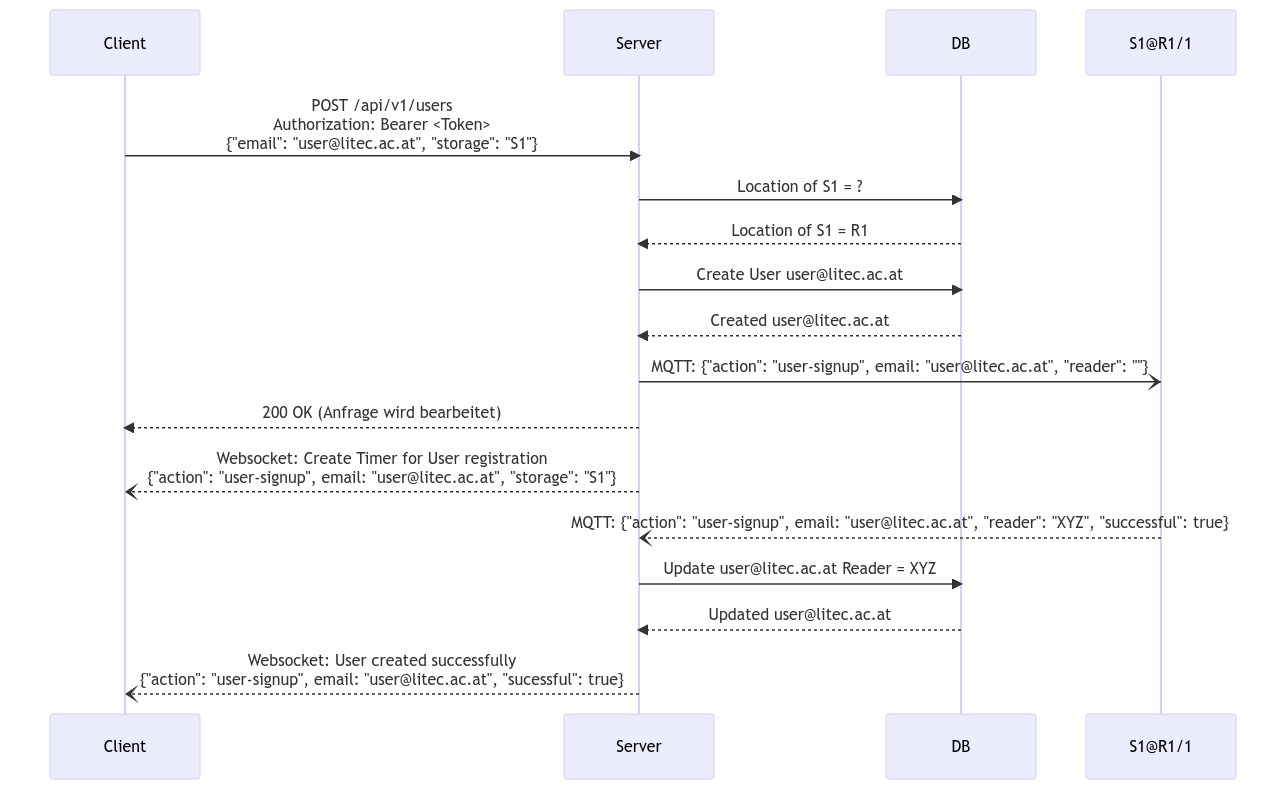
\includegraphics[width=1.15\textwidth,height=0.65\textheight]{MJ/assets/seq-diagram-ex2-usersignup.png}}
    \captionof{figure}{\centering Ablauf der Benutzerregistrierung in Form eines Sequenzdiagramms.}
    \label{fig:simulation:usersignup}
\end{center}
\vspace*{\fill}
% \begin{figure}
%     \centering
%     \makebox[1\textwidth][c]{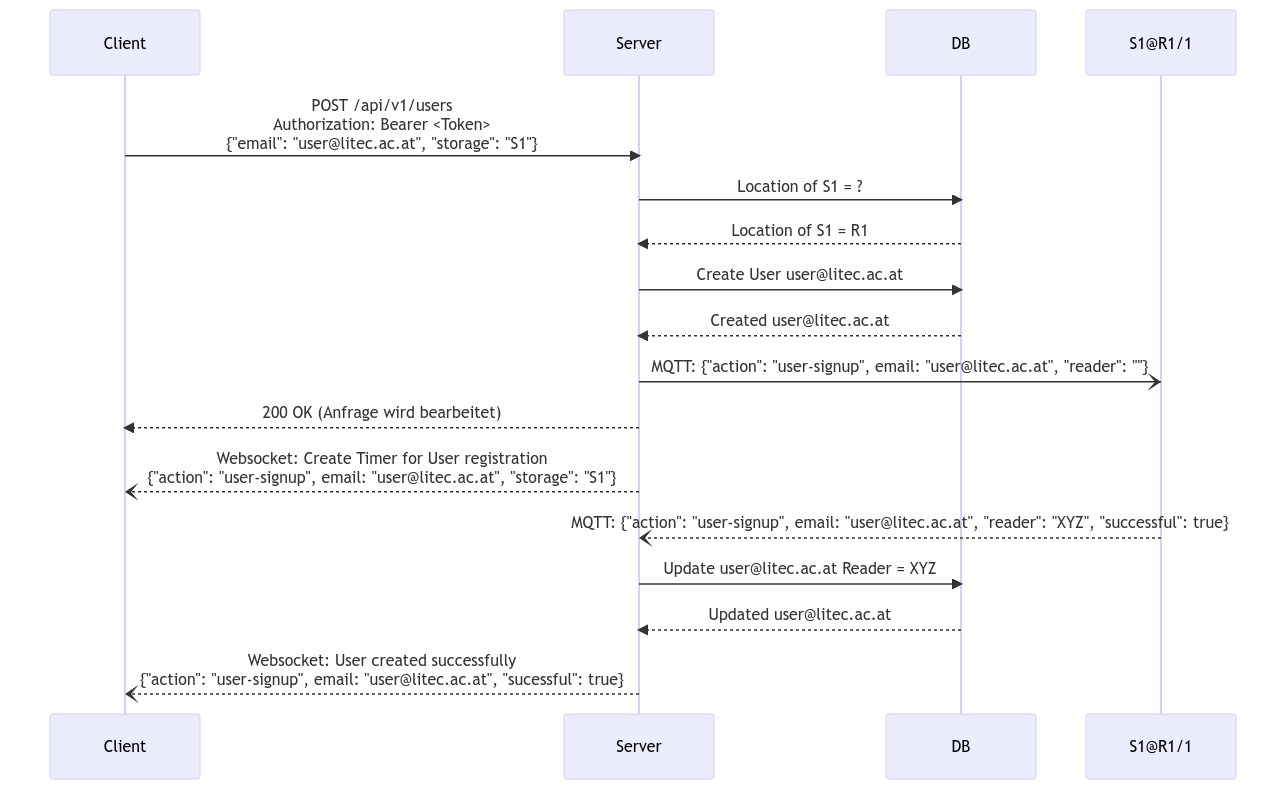
\includegraphics[width=1.35\textwidth,height=0.65\textheight]{MJ/assets/seq-diagram-ex2-usersignup.png}}
%     \caption{\centering Ablauf der Benutzerregistrierung in Form eines Sequenzdiagramms.}
%     \label{fig:simulation:usersignup}
% \end{figure}

\newpage
\subsubsection{Fallbeispiel: Client Authentifizierung}\label{sec:simulation:clientauth}
In Abbildung \ref{fig:simulation:clientauth} wird der Ablauf der Client Authentifizierung (anonym und registrierter Benutzer) dargestellt. Der erhaltene Token muss nun in allen folgenden Anfragen im HTTP-Header gesendet werden.  
\vspace*{\fill}
\begin{center}
    \makebox[1\textwidth][c]{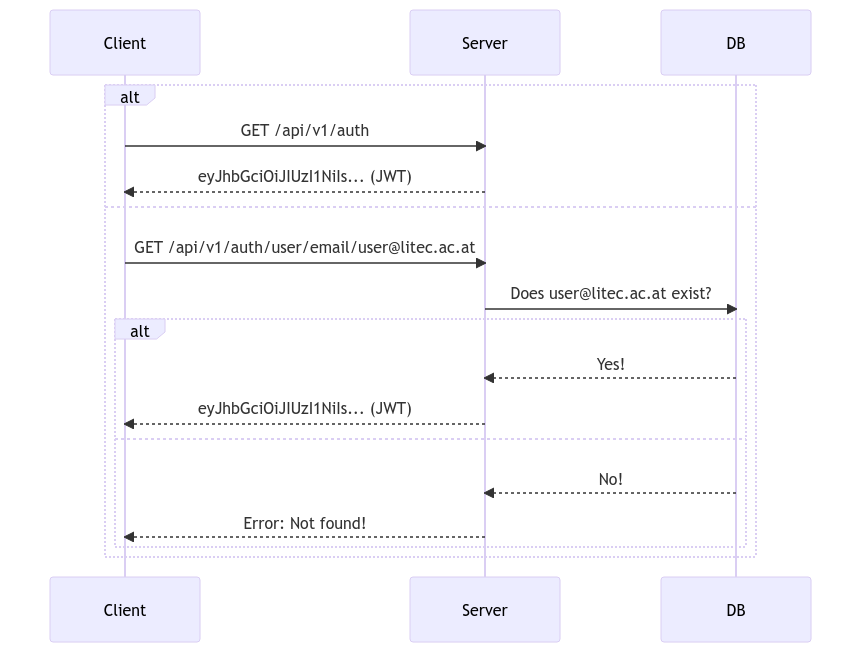
\includegraphics[width=1.2\textwidth]{MJ/assets/seq-diagram-ex3-clientauth.png}}
    \captionof{figure}{\centering Ablauf der Client Authentifzierung in Form eines Sequenzdiagramms.}
    \label{fig:simulation:clientauth}
\end{center}
\vspace*{\fill}

\newpage
\subsubsection{Fallbeispiel: Karte wird zurückgegeben}
In Abbildung \ref{fig:simulation:deposit} wird der Ablauf einer Kartenrückgabe über ein Schließfach dargestellt. Folgende Annahmen wurden getroffen: autorisierter Client (siehe Fallbeispiel \ref{sec:simulation:clientauth}) sowie erreichbarer Schließfach-Controller \textit{S1} im Raum \textit{R1}. Wird eine Karte in einem Schließfach zurückgegeben, muss zuerst überprüft werden ob diese zu dem jeweiligen Schließfach gehört. Es ist derzeit nicht vorgesehen, dass man Karten in beliebigen Schließfächern zurückgeben kann. 
\vspace*{\fill}
\begin{center}
    \makebox[1\textwidth][c]{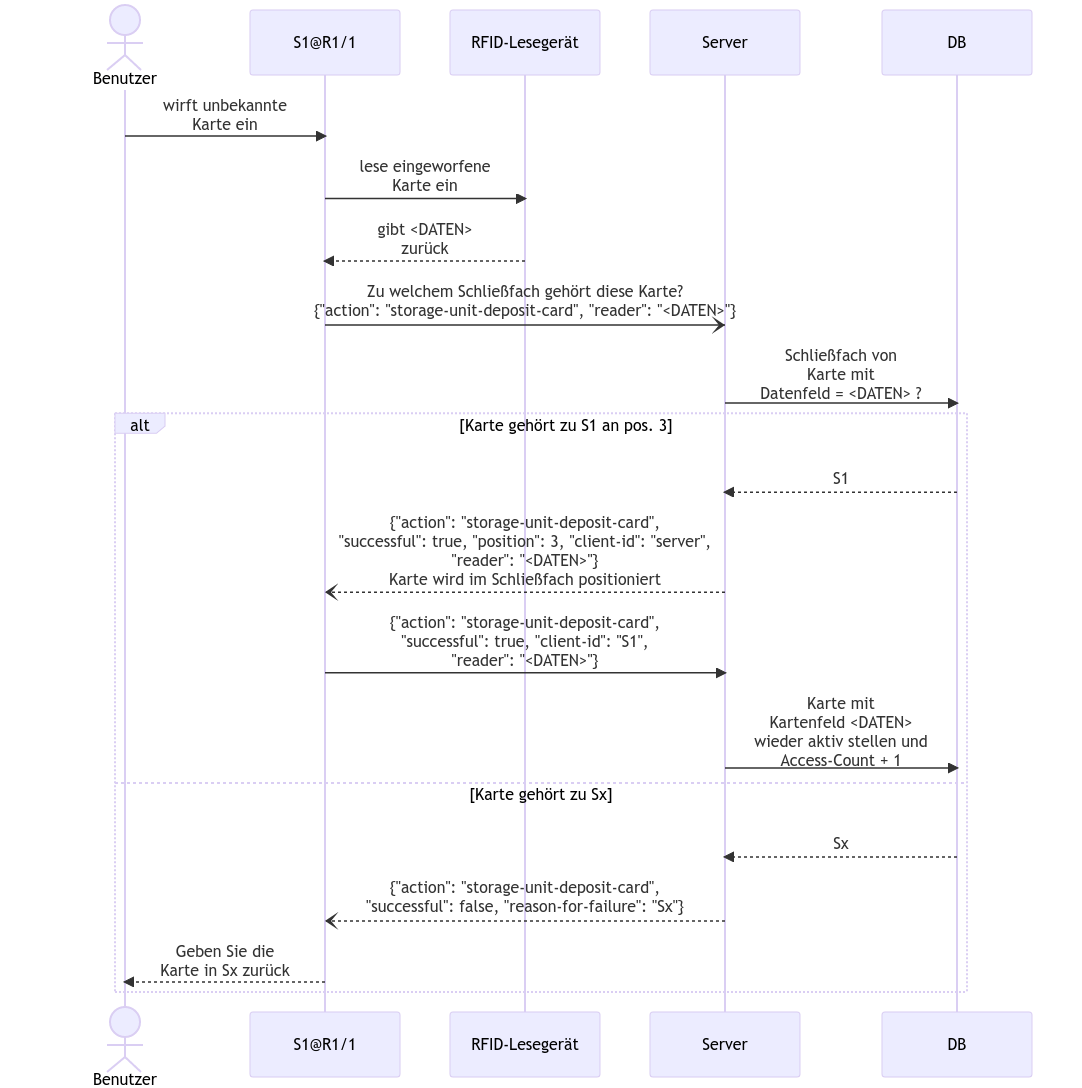
\includegraphics[width=1.25\textwidth]{MJ/assets/seq-diagram-ex4-carddeposit.png}}
    \captionof{figure}{\centering Ablauf der Kartenrückgabe in Form eines Sequenzdiagramms.}
    \label{fig:simulation:deposit}
\end{center}
\vspace*{\fill}

\newpage
\subsubsection{Fallbeispiel: Karte wird über App ausgeborgt}
In Abbildung \ref{fig:simulation:fetch:mobile} wird der Ablauf dargestellt, wie eine Karte über die App ausgeborgt wird. Folgende Annahmen wurden getroffen: autorisierter Client (siehe Fallbeispiel \ref{sec:simulation:clientauth}) mit E-Mail-Adresse \frqq{}user@litec.ac.at\flqq{}, erreichbarer Schließfach-Controller \textit{S1} im Raum \textit{R1} sowie bereits existierende und derzeit verfügbare Karte \textit{K1}. 
\vspace*{\fill}
\begin{center}
    \makebox[1\textwidth][c]{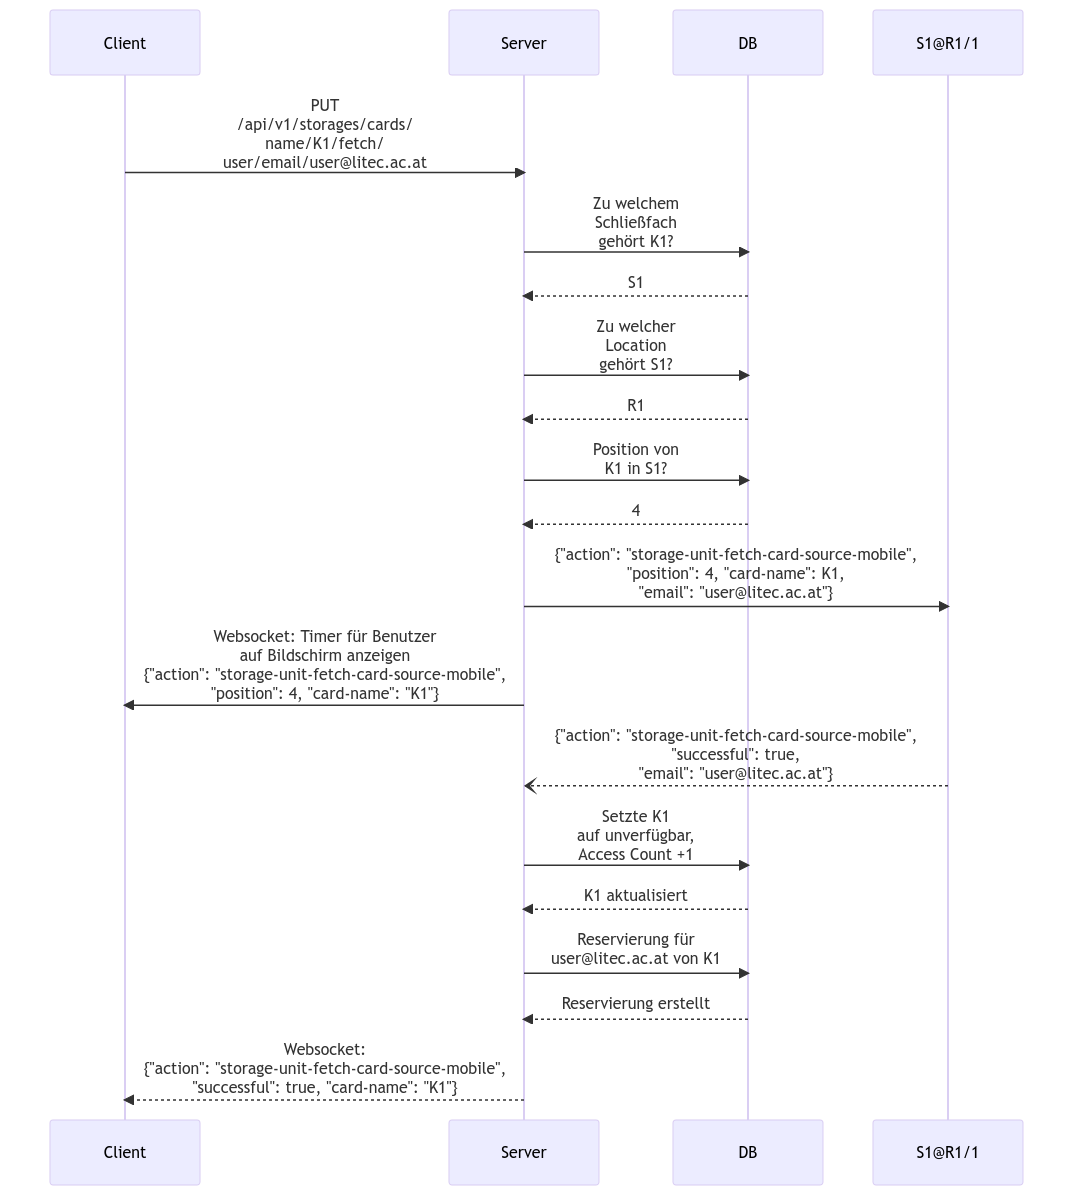
\includegraphics[width=1\textwidth]{MJ/assets/seq-diagram-ex5-fetch-mobile.png}}
    \captionof{figure}{\centering Ablauf um eine Karte über die App auszuborgen, in Form eines Sequenzdiagramms}
    \label{fig:simulation:fetch:mobile}
\end{center}
\vspace*{\fill}

\newpage
\subsubsection{Fallbeispiel: Karte wird am Schließfach Display ausgeborgt}
In Abbildung \ref{fig:simulation:fetch:terminal} wird der Ablauf dargestellt, wie eine Karte über das Schließfach-Display ausgeborgt wird. Folgende Annahmen wurden getroffen: autorisierter Client (siehe Fallbeispiel \ref{sec:simulation:clientauth}), erreichbarer Schließfach-Controller \textit{S1} im Raum \textit{R1} sowie bereits existierende und derzeit verfügbare Karte \textit{K1}. In diesem Fall ist eine mehrstufige Kommunikation zwischen Server und Schließfach-Controller notwendig da zuerst die Identität des Benutzers überprüft werden muss. Erst wenn der Benutzer seine Schlüssekarte gescannt hat und überprüft wurde, dass dieser bereits registriert ist, wird ihm die Karte zur Verfügung gestellt. 
\vspace*{\fill}
\begin{center}
    \makebox[1\textwidth][c]{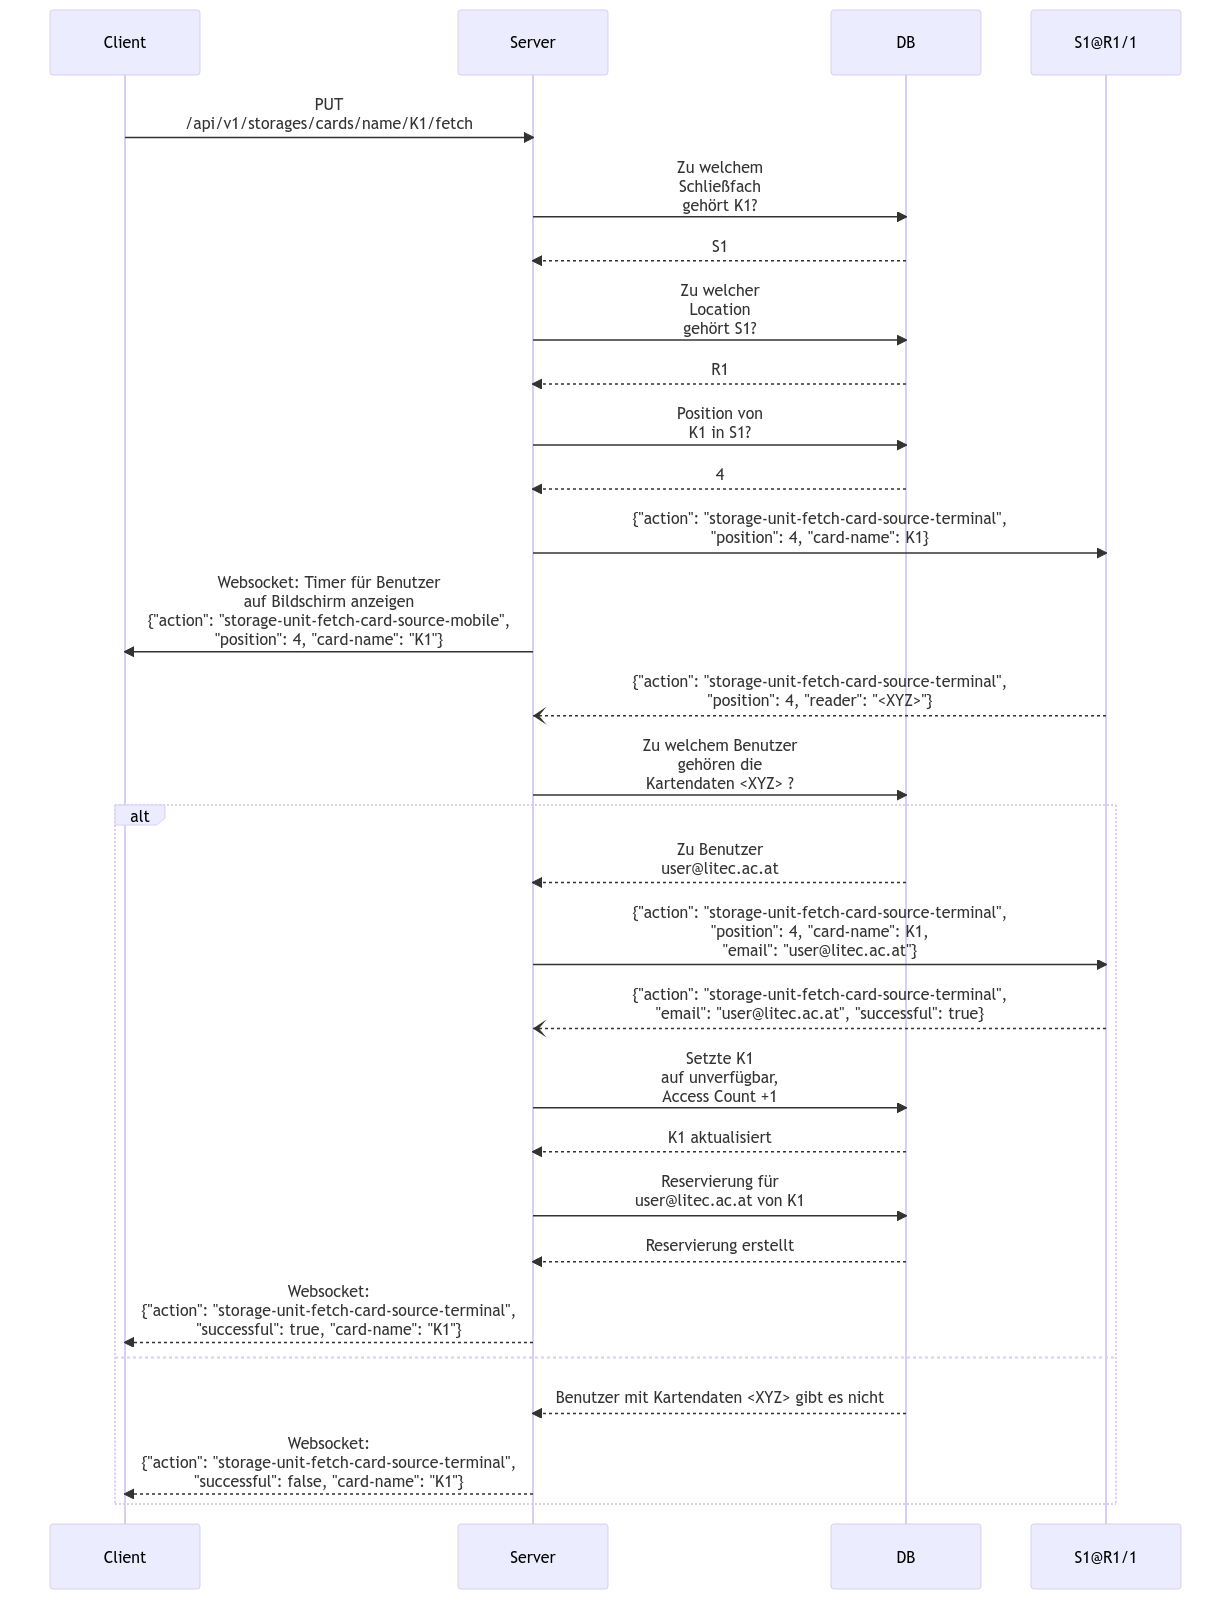
\includegraphics[width=.975\textwidth]{MJ/assets/seq-diagram-ex6-fetch-terminal.png}}
    \captionof{figure}{\centering Ablauf um eine Karte über das Schließfach-Display auszuborgen, in Form eines Sequenzdiagramms}
    \label{fig:simulation:fetch:terminal}
\end{center}
\vspace*{\fill}

\newpage
\subsubsection{Fallbeispiel: Ping eines Schließfach-Controllers}
In Abbildung \ref{fig:simulation:ping} wird der Ablauf eines Pings, also die Frage seitens eines Clients ob ein gegebener \gls{storageController}, \textit{S1} im Raum \textit{R1}, erreichbar ist, dargestellt.
\vspace*{\fill}
\begin{center}
    \makebox[1\textwidth][c]{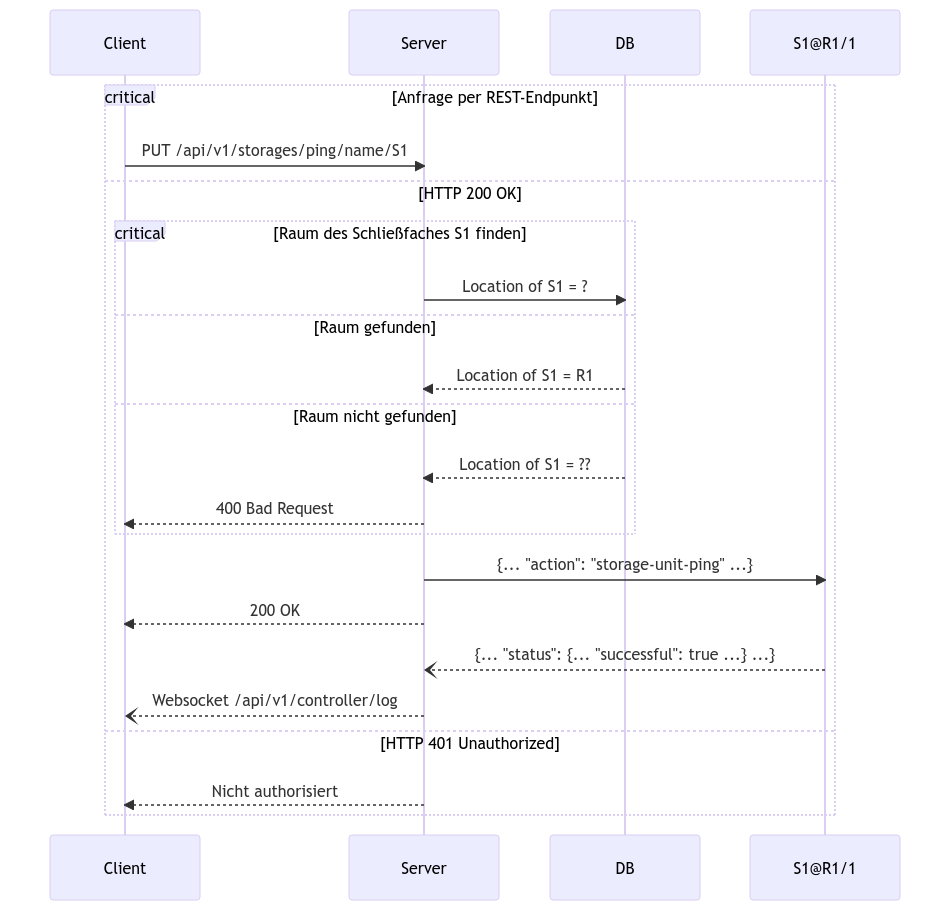
\includegraphics[width=1.15\textwidth]{MJ/assets/seq-diagram-ex1-ping.png}}
    \captionof{figure}{\centering Ablauf der \textit{Ping} Abfrage in Form eines Sequenzdiagramms.}
    \label{fig:simulation:ping}
\end{center}
\vspace*{\fill}

\newpage
\subsection{Middleware Framework \textit{Meridian}}\label{sec:impl:merdian}
Im diesem Abschnitt wird das für die vorliegende Implementierung entworfene Middleware Framework, \textit{Meridian}, vorgestellt. Allgemeine Informationen zu Middleware finden sich im Anschnitt \ref{sec:theory:middleware}. \textit{Meridian} wurde derart generalisiert, sodass es für die beiden übergeordneten Schnittstellen zum Einsatz kam. Konkret wurde es auf Seite der Benutzer-Schnittstelle für alle \acrshort{rest}-API-Endpunkte zur Authentifizierung, zum Logging sowie zum asynchronen Datenaustausch mittels Websockets verwendet. Auf Seite der \gls{storageController}-Schnittstelle wurde Merdian ebenfalls dazu verwendet, den asynchronen Datenaustausch zwischen Client und Server mittels Websockets, in Kombination mit dem im nachfolgenden Abschnitt (\ref{sec:impl:event-handler-dispatcher-system} \nameref{sec:impl:event-handler-dispatcher-system}), näher erläuterten \textit{Controller}-Framework zu erleichtern.

\subsubsection{Middleware in der Client-Schnittstelle}
In Abbildung \ref{fig:middleware} wird der Ablauf des in der Client-Schnittstelle verwendeten Middleware Frameworks veranschaulicht. Der HTTP Origin-Check, HTTP Method-Check sowie HTTP Header-Check werden von einer Bibliothek, namens \textit{Gorilla-Handlers}, welche Bestandteil von dem Go-Web-Framework, \textit{Gorilla} ist (mehr Informationen dazu im Abschnitt \ref{sec:tech:gorilla}), behandelt. Der weitere Ablauf wird von Merdian verwaltet.\medskip

\noindent
Nachdem der Benutzer-Token im Authorization Schritt überprüft wurde, wird der eigentliche \gls{resourceHandler} des vom Client geforderten Endpunktes aufgerufen. Je nachdem welchen Rückgabewert dieser \gls{resourceHandler} erzeugt wird dem Client entweder als Antwort der Statuscode sowie etwaige Daten zurückgegeben oder im Falle eines aufgetretenen Fehlers welcher mit einem \gls{storageController} in Verbindung steht, dieser über die zugehörige Websocket Verbindung näher erläutert. Zuletzt wird die bearbeitete Anfrage protokolliert (derzeit Konsole).
\vspace*{\fill}
\begin{center}
    \makebox[\textwidth][c]{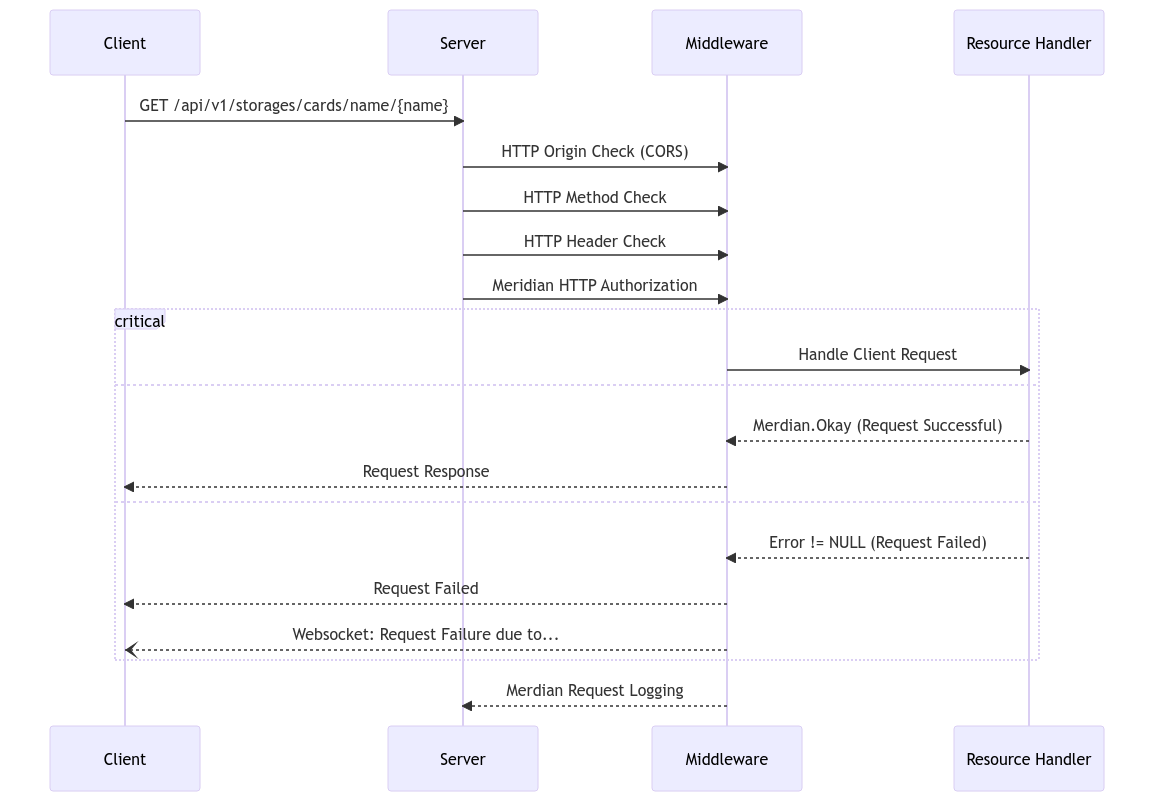
\includegraphics[width=1.2\textwidth]{MJ/assets/seq-diag-middleware-v2.png}}
    \captionof{figure}{\centering Middleware Ablauf der Client-Schnittstelle in Form eines Sequenzdiagramms}
    \label{fig:middleware}
\end{center}
\vfill

\newpage
\subsection{Multiplexing von \acrshort{sscp}-Nachrichten: \textit{Observer}}\label{sec:impl:multiplexing}
In diesem Abschnitt wird die Behandlung von Ereignissen innerhalb der \gls{storageController}-Schnittstelle, konkret die Weiterleitung der \acrshort{sscp}-Nachrichten zu den richtigen Handlern, näher erläutert. Ausgangslage: die \gls{storageController}-Schnittstelle steht via MQTT mit allen Schließfach-Controllern in Verbindung. Um die eingehenden Nachrichten richtig nach Absender, sowie Aktion zu unterscheiden und einzuordnen, werden \textit{alle} eingehenden \acrshort{sscp}-Nachrichten vom \textit{Observer} Framework untersucht und an den richtigen Handler, der die Anfrage weiter bearbeitet, weitergeleitet.\bigskip

\noindent
Das Verhalten des Observes kann mit dem eines Postverteilzentrums, welches Pakete an die weiteren Zusteller verteilt, verglichen werden. Der Observer agiert ähnlich, indem er zu Beginn den \acrshort{sscp}-Header der Nachricht deserialisert. Nachdem dieser in der entsprechenden Go-Struktur vorliegt, wird der Absender der Nachricht überprüft. Dieser Schritt ist notwendig da die \gls{storageController} Schnittstelle auf das Topic der Schließfächer fokusiert (MQTT Subscribe) ist und gleichzeitig darauf Nachrichten veröffentlicht (MQTT Publish). Aus diesem Grund wurde die \textit{Client-Id} in das \acrshort{sscp}-Protokoll integriert, da man ansonsten nicht weiß, wer die empfangene Nachricht gesendet hat. Dies ist ein weiterer Grund für die Notwendigkeit einer eindeutigen \textit{Client-Id}. Ändert ein \gls{storageController} die Client-Id nicht auf einen eindeutigen Wert (ein \gls{storageController} vergisst zb. die vom Server erhaltene Client-Id auf dessen eigene zu ändern) wird diese Nachricht vom Observer schlichtweg ignoriert.\\ Nachdem der Observer die Client-Id überprüft hat und eruiert hat, dass die eingehende Nachricht nicht vom Server stammt, sondern eine Antwort eines \gls{storageController}'s ist, wird die \textit{Aktion} der Nachricht weiter untersucht. Jede Aktion ist mit einem Aktions-Handler, also einem Event-Handler, welcher bei dem Empfang einer solchen Nachricht aufgerufen wird, assoziiert. Nachdem der passende Aktions-Handler zur sich im Header befindlichen Aktion gefunden wurde, wird diesem die gesamte Nachricht übergeben, welche dann spezifisch für jeden Handler ausgewertet wird.
\newpage
\vfill
\begin{lstlisting}[style=goMono,caption={\centering Weiterleitung von eingehenden \acrshort{sscp}-Nachrichten an den damit assoziierten Ereignis-Handler},label={lst:impl:observer:ex1}]
return func(client mqtt.Client, msg mqtt.Message) {
  go func(s *meridian.StaticMqttReporter) {
    if len(string(msg.Payload())) > (1 << 10) { %\mono{\color{magenta}(1)}%
      ...
      return
    }
    header := &controller.Header{}
    err := json.Unmarshal(msg.Payload(), header) %\mono{\color{magenta}(2)}%
    if err != nil {
      ...
      return
    }
    if header.ClientId == c.ClientId { %\mono{\color{magenta}(3)}%
      ...
      return
    }

    switch header.Action { %\mono{\color{magenta}(4)}%
    case controller.ActionStorageUnitPing:
      s.Reporter(c.PingStorageUnitHandler)(msg) %\mono{\color{magenta}(5)}%
      return
    case controller.ActionStorageUnitNewCard:
      s.Reporter(c.StorageUnitAddCardHandler)(msg)
      return
    case controller.ActionStorageUnitDeleteCard:
      s.Reporter(c.DeleteCardHandler)(msg)
      return
    case controller.ActionStorageUnitFetchCardSourceMobile:
      s.Reporter(c.FetchCardKnownUserHandler)(msg)
      return
    case controller.ActionStorageUnitFetchCardSourceTerminal:
      s.Reporter(c.FetchCardUnknownUserHandler)(msg)
      return
    case controller.ActionUserSignup:
      s.Reporter(c.SignUpUserHandler)(msg)
      return
    case controller.ActionStorageUnitDepositCard:
      s.Reporter(c.DepositCardHandler)(msg)
      return
    }
  }(s)
}
\end{lstlisting}
\vfill
\newpage
\subsubsection{Vom \gls{storageController} zum Benutzer}
Im obigen Listing (\ref{lst:impl:observer:ex1}) befindet sich ein gekürzter Ausschnitt des Observer-Frameworks, das den oben textuell beschriebenen Algorithmus abbildet. In \mono{\color{magenta}(1)} werden zusätzlich alle eingehenden Nachrichten abgelehnt, die größer als $\texttt{(1<<10)}=2^{10}=1024$ Bytes sind (Zeichen in Go, auch bekannt unter \textit{runes}, sind jeweils 1 Byte groß). Als nächstes \mono{\color{magenta}(2)} wird der Nachrichten-Header mit der eingebauten \mono{json.Unmarshal} Funktion deserialisiert. Schritt \mono{\color{magenta}(3)} überprüft ob die aktuelle Nachricht vom Server (\mono{c.ClientId}) oder von einem \gls{storageController} stammt. Falls diese vom Server stammt wird die Nachricht abgelehnt. Nun \mono{\color{magenta}(4)} wird der, mit der in der Nachricht, spezifizierten Aktion, assoziierte Handler aufgerufen. Jedoch wird dieser Handler nicht direkt aufgerufen \mono{\color{magenta}(5)} sondern indirekt mit Hilfe des im Abschnitt \ref{sec:impl:merdian} (\nameref{sec:impl:merdian}) beschriebenen Middleware-Frameworks, \textit{Meridian}. Wie in \mono{\color{magenta}(5)} ersichtlich, wird eine Referenz auf den eigentlichen Aktions-Handler übergeben und vom \textit{Reporter} aufgerufen. Dieser verbindet die Benutzer-Schnittstelle mit der Schließfach-Controller-Schnittstelle, indem dieser, die Informationen, welche der Aktions-Handler zurückgibt, über die Websocket Verbindung veröffentlicht. 

\newpage
\subsection{Event Handler-- und Dispatcher Framework: \textit{Controller}}\label{sec:impl:event-handler-dispatcher-system}
Wie bereits im Abschnitt \ref{sec:impl:multiplexing} (\nameref{sec:impl:multiplexing}) näher erläutert, ist jede \acrshort{sscp}-Aktion mit einem Handler, also einer Funktion welche aufgerufen wird sobald eine Nachricht mit der jeweiligen Aktion empfangen wird, assoziiert.\bigskip

\noindent
Dies ist jedoch nur eine Seite der Münze. Aktionen müssen schlussendlich zuerst angestoßen werden, bevor sie behandelt werden können. Daher ist jede Aktion auch mit einem sogenannten Dispatcher, also einem Auslöser, assoziiert. Der Server ist der aktive Teil der Kommunikation, und der \gls{storageController} der passive. Damit ist gemeint, dass der Server die Kommunikation beginnt und der \gls{storageController} darauf antwortet. Dafür gibt es bisher 1 Ausnahme: die (im Abschnitt \ref{sec:impl:storageController:actions} beschriebene) \textit{Deposit} Aktion. In diesem Fall initiiert der jeweilige \gls{storageController} die Kommunikation mit dem Server, da eine Karte zurückgegeben wurde.\bigskip

\noindent
In folgenden Beispielen wird (wie im Abschnitt \ref{sec:impl:sideeffects} \nameref{sec:impl:sideeffects}, bereits näher erläutert wurde) auch veranschaulicht, dass Daten in der Datenbank erst dann verändert werden wenn eine Aktion vollständig abgeschlossen ist (also im Handler der Antwort-Nachricht).  

\newpage
\subsubsection{Fallbeispiel: Benutzer Registrierung}
\begin{lstlisting}[style=goMono, caption={\centering Dispatcher, um dem System einen neuen Benutzer hinzuzufügen}, label={lst:impl:controller:ex1}]
func (self *Controller) SignUpUserDispatcher %\mono{\color{magenta}(1)}%
    (storageName, location, email string)    %\mono{\color{magenta}(2)}%
    (*SerializableUserMessage, error) {      %\mono{\color{magenta}(3)}%
  
  id := uuid.New().String()

  kickoff := NewSerializableUserMessage(Header{Id: id, %\mono{\color{magenta}(4)}%
    ClientId: self.ClientId, Action: ActionUserSignup},
    User{Email: &email}, Status{})

  buf, err := json.Marshal(kickoff)  %\mono{\color{magenta}(5)}%
  if err != nil {
    return nil, err
  }

  token := self.Publish(  %\mono{\color{magenta}(6)}%
    storageName + "@" + location + "/1"), 2, false, buf) %\mono{\color{magenta}(7)}%
  
  err := token.Error()
  if err != nil {
    return nil, err
  }

  return &kickoff, nil %\mono{\color{magenta}(8)}%
}
\end{lstlisting}
Das obige Listing (\ref{lst:impl:controller:ex1}) stellt den in der vorliegenden Implementierung verwendeten Ereignis-Dispatcher um dem System einen neuen Benutzer hinzuzufügen, dar. Der Ereignis-Dispatcher \mono{\color{magenta}(1)} wird aufgerufen, sobald der Client einen neuen Benutzer über die Client-Schnittstelle hinzufügen möchte: \mono{POST /api/v1/users}.
\newpage
Um einen Benutzer zu erzeugen, muss der Client, im JSON-Body der Anfrage, mindestens eine E-Mail-Adresse des anzulegenden Benutzers sowie den Namen des Schließfach-Controllers, an welchen er sich registrieren soll, übergeben:
\begin{lstlisting}[style=goMono,caption={Benötigter JSON-Body um einen Benutzer anzulegen}]
{
    "email": "card_storage_user@litec.ac.at",
    "storage": "S1",
    "privileged": false
}
\end{lstlisting}
Das Feld \mono{privileged} entscheidet ob der neue Benutzer Administrator-Rechte haben soll oder nicht. Diese Feld ist optional und standardmäßig auf \mono{false} gesetzt. Bevor der Ereignis-Dispatcher aufgerufen wird, wird der zum Schließfachnamen zugehörige Raum (location) von der Datenbank abgefragt und dem Ereignis-Dispatcher im Aufruf \mono{\color{magenta}(2)} übergeben. Im nächsten Schritt wird eine \acrshort{sscp}-Nachricht mit den übergebenen Daten initialisiert \mono{\color{magenta}(4)} und als Bytefolge \mono{\color{magenta}(5)} serialisiert. Diese Nachricht wird an das \gls{storageController} Topic gesendet \mono{\color{magenta}(6)}, das sich aus dem \gls{storageController}-Namen und dessen Location \mono{\color{magenta}(7)} zusammensetzt. Nachdem die \acrshort{sscp}-Nachricht an das jeweilige Topic gesendet wurde, wird das gesendete Objekt an den Aufrufer, also den API-Endpunkt-Handler zurückgegeben. Das Objekt wird an den API-Endpunkt-Handler zurückgegeben \mono{\color{magenta}(8)}, und dort auf dem Benutzer-Websocket\\ \mono{/api/v1/users/log} veröffentlicht, sodass die Kollegen welche für die grafische Oberfläche zuständig sind, einen Timer implementieren konnten um den Benutzer zu signalisieren, dass dieser seine Schlüsselkarte an den \acrshort{rfid}-Leser des Schließfaches halten möge.\bigskip

\noindent
Ähnlich funktioniert dieser Ablauf wenn eine Karte ausgeborgt werden soll: 
\begin{description}
\item API-Endpunkt Anfrage, 
\item Dispatcher wird aufgerufen, 
\item Card-Objekt wird auf \mono{/api/v1/storages/cards/log} veröffentlicht, sodass die Kollegen deren Timer anzeigen können um den Benutzer zu signalisieren, dass sich dieser die Karte abholen soll, 
\item Benutzer holt sich Karte, 
\item Schließfach-Controller sendet Antwort an Server, 
\item Server ruft zugehörigen Handler auf, 
\item Daten zu jeweiliger Karte werden in der Datenbank aktualisiert, 
\item Clients werden über Controller-Websocket \mono{/api/v1/controller/log} darüber informiert, dass eine Karte ausgeborgt wurde.     
\end{description}
Dieser Prozess welcher abläuft, wenn eine Nachricht vom \gls{storageController} beantwortet wird, wird anhand des nächsten Listings veranschaulicht und näher erläutert.  
% Dieser konkrete Ereignis-Dispachter gibt die 
\begin{lstlisting}[style=goMono, caption={\centering Handler, um dem System einen neuen Benutzer hinzuzufügen}, label={lst:impl:controller:ex2}]
func (self *Controller) SignUpUserHandler %\mono{\color{magenta}(1)}%
    (message mqtt.Message) (error, *meridian.Ok) { %\mono{\color{magenta}(2)}%

  m := SerializableUserMessage{} %\mono{\color{magenta}(3)}% 
  err := json.Unmarshal(message.Payload(), &m) %\mono{\color{magenta}(4)}% 
  if err != nil {
    return err, nil %\mono{\color{magenta}(10)}% 
  }

  if m.Successful { %\mono{\color{magenta}(10)}% 
    err := self.DB. %\mono{\color{magenta}(5)}% 
      Model(&model.User{}). %\mono{\color{magenta}(6)}% 
      Where("email = ?", m.Email). %\mono{\color{magenta}(7)}% 
      Update("reader_data", m.ReaderData).Error %\mono{\color{magenta}(8)}% 
    if err != nil {
      return err, nil
    }
  }

  return nil, meridian.Okay(string(message.Payload())) %\mono{\color{magenta}(9)}% 
}
\end{lstlisting}
Das obige Listing (\ref{lst:impl:controller:ex2}) stellt den in der vorliegenden Implementierung verwendeten Event-Handler \mono{\color{magenta}(1)}, um Benutzer dem System hinzuzufügen, dar. Dieser wird aufgerufen wenn ein \gls{storageController} eine vom Server (siehe vorheriges Listing \ref{lst:impl:controller:ex1}) gesendete Anfrage beantwortet. Die Event-Handler wurden mit der im Abschnitt \ref{sec:impl:merdian} (\nameref{sec:impl:merdian}) näher erläuterten Middleware Bibliothek, Meridian, integriert. Aus diesem Grund haben alle Event-Handler  \mono{\color{magenta}(2)} dieselbe Struktur: tritt ein Fehler im Event-Handler auf, wird dieser als 1. Rückgabewert zurückgegeben \mono{\color{magenta}(10)} wobei der 2. Rückgabewert, welcher sonst die empfangene Nachricht\\ \mono{message.Payload()} beinhaltet, leer bleibt (null pointer). Sofern alles korrekt abgelaufen ist, ist der error Rückgabewert leer (null) und es wird stattdessen die empfangene Nachricht zurückgegeben. Die empfangene Nachricht wird an der sich im Listing \ref{lst:impl:observer:ex1} befindlichen \mono{Reporter} Middleware zurückgegeben, in welcher die Nachricht wieder auf dem Client-Websocket \mono{/api/v1/controller/log} veröffentlicht wird, sodass die Clients über die neue Benutzer Registrierung verständigt werden.\bigskip

\noindent
Eine vom Schließfach-Controller gesendete Antwort-Nachricht könnte folgendermaßen aussehen:
\begin{lstlisting}[style=goMono,label={lst:impl:eventhandlerdispatcher:ex5},caption={\centering Antwort: Ausformulierte JSON-Repräsentation einer Benutzerregistrierung}]
{
   "message-id": "786fcea6-afe0-11ed-afa1-0242ac120002",
   "client-id": "S1",   
   "action": "user-signup",
   "status": {
      "successful": true,
      "reason-for-failure": ""
   },
   "user": {
     "email": "card_storage_user@litec.ac.at"
     "reader": "YTFiMmMzZDRlZg=="
   }
}
\end{lstlisting}
Hier wird nun der Ablauf des Event-Handlers im Listing \ref{lst:impl:controller:ex2} weiter erklärt. Die empfangene Nachricht \mono{msg.Payload()} wird in eine Go-Struktur \mono{\color{magenta}(3)} deserialisiert \mono{\color{magenta}(4)}. Danach werden die Änderungen in die Datenbank geschrieben \mono{\color{magenta}(5)}. Dies erfolgt mit folgender Syntax: zuerst muss GORM der Typ, welcher aktualisiert werden soll bekannt gegeben werden \mono{\color{magenta}(6)}. Danach wird mit einer \textit{Where} Klausel \mono{\color{magenta}(7)} der bereits im Endpunkt-Handler erstellte (uninitalisierte) Benutzer mit dessen Schlüsselkarten Daten aktualisiert \mono{\color{magenta}(8)}. Falls ein Fehler aufgetreten ist, wird dieser per Websocket zurückgegeben, sodass der Client diese dem Benutzer präsentieren kann und die Anfrage muss erneut gestellt werden.

\subsubsection{Fehlgeschlagene Aktionen}
Angenommen die im Listing \ref{lst:impl:eventhandlerdispatcher:ex5} veranschaulichte Antwort wäre fehlgeschlagen:
\begin{lstlisting}[style=goMono,label={lst:impl:eventhandlerdispatcher:ex6},caption={\centering Antwort: Ausformulierte JSON-Repräsentation einer Benutzer Registrierung}]
{
   "message-id": "786fcea6-afe0-11ed-afa1-0242ac120002",
   "client-id": "S1",   
   "action": "user-signup",
   "status": {
      "successful": false,
      "reason-for-failure": "unable to reach rfid scanner"
   },
   "user": {
     "email": "card_storage_user@litec.ac.at"
     "reader": ""
   }
}
\end{lstlisting}
Der Schließfach-Controller meldet in diesem Fall, dass die Anfrage nicht erfüllt werden konnte, da er den \acrshort{rfid}-Leser nicht aktivieren konnte. Dies ist einerseits an dem \mono{successful} Flag im \mono{status} flag ersichtlich und darin, dass es einen \mono{reason-for-failure} gibt. In diesem Fall wird, wie in Listing \ref{lst:impl:controller:ex2} ersichtlich, die Datenbank nicht aktualisiert \mono{\color{magenta}(10)} (da \mono{successful == false}) und die Nachricht per Websockets an den Client übergeben, sodass dieser die Fehlermeldung, nämlich, dass der Kartenlesevorgang nicht gestartet werden konnte, benutzerfreundlich ausgeben kann.

\subsubsection{Zusammenspiel zwischen \textit{Observer}, \textit{Meridian} und \textit{Controller} Frameworks}
Im genannten Listing \ref{lst:impl:controller:ex2} wird ebenfalls die Verbindung zum im Abschnitt \ref{sec:impl:multiplexing} erklärten Observer Framework hergestellt \mono{\color{magenta}(9)}. Im Listing \ref{lst:impl:observer:ex1}, in welchem die einzelnen Event-Handler auf Basis der empfangenen Aktion aufgerufen werden, wird der Rückgabewert des Event-Handlers \mono{\color{magenta}(2)} dem Middleware Framework, Meridian, übergeben. Dieses stellt wiederum die Verbindung zur Benutzer-Schnittstelle her indem es den Rückgabewert \mono{\color{magenta}(9)} auf dem Schließfach-Controller Websocket \mono{/api/v1/controller/log} veröffentlicht.

 \newpage
\section{Simulation des Gesamtsystems}\label{sec:impl:simulators}
Ein Programm, in diesem Fall ein Softwaresystem, sollte vor dessen Einsatz möglichst gründlich getestet werden. Um das im Zuge dieser Arbeit entstandene System zu testen, reichten einfache Unit-Tests nicht aus. Daher musste das gesamte System zuerst simuliert werden, bevor es getestet werden konnte. Dazu wurden zwei Simulatoren entwickelt, welche einerseits die Kommunikation zwischen Benutzer und Server, also eine übliche Client-Server Architektur und andererseits zwischen Schließfächer und Server, simulieren.\bigskip

\noindent
Diese Simulatoren werden ausserhalb des Kernsystems, also ausserhalb der im Abschnitt \ref{sec:impl:docker} näher erläuterten, containerisierten Umgebung des Systems, zur Verfügung gestellt. Um diese zu starten wird eine Go-Entwicklungsumgebung benötigt. Mehr Informationen zur benötigten Software, sowie Informationen zur Konfiguration des vorliegenden Systems, lassen sich dem im Abschnitt \ref{sec:apdx:user-guide:mj} befindlichen Benutzerhandbuch entnehmen. 

\subsection{Client-Simulator}\label{sec:impl:simualtion:client}
Der Client-Simulator simuliert die von den Kollegen umgesetzten Anwendungen, um die Client-Schnittstelle des Servers schnell und effizient testen zu können. Dieser wurde hauptsächlich zu Testzwecken entwickelt, um nicht ständig die \acrshort{http} Anfragen manuell tippen zu müssen. Die Anwendung wurde in Form einer textbasierten Kommandozeilen Anwendung umgesetzt. Der Ablauf der Anwendung funktioniert folgendermaßen
\begin{description}
\item[Initialisierung] Bevor der Simulator bereit ist, die vom Benutzer geforderten Anfragen auszuführen, muss dieser initialisiert werden. Zur Initialisierung zählen folgende Schritte: 
\begin{description}
    \item[Authentifizierung als Anonym] Der Client-Simulator authentifiziert sich an der Client-Schnittstelle als Anonymer Benutzer um den nächsten Initialisierungs-Schritt durchführen zu können. \textit{Hinweis}: Selbstverständlich kann sich der Benutzer des Simulators auch als registrierter Benutzer des Systems authentifizieren. Die anfängliche Authentifizierung als Anonym wurde nur zur automatischen Herstellung der Websocket Verbindung am Programmstart durchgeführt. Sobald ein neuer Benutzer erfolgreich authentifiziert ist, wird fortan dessen Authentifizierungs-Token verwendet.
    \item[Websocket Verbindung herstellen] Der Client-Simulator verbindet sich mit allen verfügbaren Websockets und gibt die empfangenen Nachrichten aus. Nähere Informationen bezüglich dem Zusammenspiel zwischen Websockets und der Client-Authentifizierung finden sich im Abschnitt \ref{sec:privilegesAndAuthorization} (\nameref{sec:privilegesAndAuthorization}).  
\end{description}
\item[Benutzer Anweisungen ausführen] Sobald die Initialisierung abgeschlossen ist, ist der Simulator bereit, Anfragen auszuführen. Die Benutzeroberfläche des Client-Simulators ist sehr einfach aufgebaut: jeder Aktion wurde eine eindeutige Zahl zugewiesen, die der Benutzer aus der Übersicht abliest und über das Nummernfeld auf seiner Tastatur eingibt. Falls eine Anfrage zusätzliche Parameter, etwa einen Kartennamen oder eine Benutzer E-Mail-Addresse, benötigt, müssen diese ebenfalls vom Benutzer des Client-Simulators eingegeben werde. Falls zwischenzeitlich eine Nachricht von einem Websocket empfangen wird, wird diese auch ausgegeben. %Dies steht jedoch keinesfalls im Konflikt zu einer Benutzer Eingabe, welche gerade stattfinden könnte. 
\noindent Im nachfolgenden Listing (\ref{lst:impl:simulator:client:start}) ist die Benutzeroberfläche und alle verfügbaren Operationen welche der Simulator unterstützt, veranschaulicht. 
\end{description}
\begin{lstlisting}[style=goMono, caption={Client-Simulator beim Programmstart}, label={lst:impl:simulator:client:start}]
client-simulator: 2023/02/19 13:28:30 200 OK %\mono{\color{magenta}(1)}%
client-simulator: 2023/02/19 13:28:30 token: eyJhbGcid...

listening: wss://localhost:7171/api/v1/controller/log %\mono{\color{magenta}(2)}%
listening: wss://localhost:7171/api/v1/storages/log
listening: wss://localhost:7171/api/v1/storages/cards/log
listening: wss://localhost:7171/api/v1/reservations/log
listening: wss://localhost:7171/api/v1/users/log

-1...StorageUnit:  Ping %\mono{\color{magenta}(3)}%
-2...StorageUnit:  Focus
-4...StorageUnit:  GetUnfocused
 0...StorageUnit:  Update
 1...StorageUnit:  New
 2...StorageUnit:  Delete
 3...StorageUnit:  GetAll
 4...StorageUnit:  GetByName
 5...Card:         New
 6...Card:         Delete
 7...Card:         GetAll
 8...Card:         GetByName
 9...Card:         Update
-3...Card:         Fetch
10...User:         New
11...User:         Update
12...User:         GetAll
13...User:         GetByName
14...User:         Delete
15...Reservation:  GetAll
16...Reservation:  GetByCardName
17...Reservation:  GetByUserEmail
18...Reservation:  New
19...Reservation:  Delete
20...Reservation:  Update
21...Authenticate: UserEmail
22...Authenticate: Anonymous
>>> 3       %\mono{\color{magenta}(4)}%
client-simulator: 2023/02/19 13:28:43 200 OK
client-simulator: 2023/02/19 13:28:43 [ %\mono{\color{magenta}(5)}% 
  {
    "name": "S1",
    "location": "L1",
    "address": "schule.local",
    "capacity": 10,
    "cards": []
  },
  {
    "name": "S2",
    "location": "L2",
    "address": "schule.local",
    "capacity": 10,
    "cards": []
  }
]
>>> %$\square$% %\mono{\color{magenta}(6)}%
\end{lstlisting}
Sobald der Client-Simulator gestartet wird, läuft der oben beschriebene Initialisierungs Vorgang, siehe \mono{\color{magenta}(1)} und \mono{\color{magenta}(2)}, ab. Nachdem dieser abgeschlossen ist wird eine Übersicht über die unterstützten Operationen \mono{\color{magenta}(3)} und deren zugehöriger numerischer Code ausgegeben, sodass der Benutzer des Client-Simulators weiß, wie dieser zu verwenden ist. \textit{Hinweis}: Diese Legende an unterstützten Operationen kann jederzeit wieder ausgegeben werden, indem \keys{\return} (Enter) auf der Tastatur gedrückt wird. Wählt der Benutzer eine Aktion aus, in diesem Fall die Aktion \textit{3}, um alle im System vorhandenen Schließfächer auszugeben \mono{\color{magenta}(4)}, sendet der Client-Simulator die passende HTTP-Anfrage an den Server und gibt dessen JSON-Antwort \mono{\color{magenta}(5)}, benutzerfreundlich formatiert, aus. Der Client-Simulator ist nun für die nächste Anfrage bereit \mono{\color{magenta}(6)}.

% Im Listing \ref{lst:impl:simulator:client:start}

\subsection{Controller-Simulator}
Der Controller-Simulator simuliert das Verhalten eines \gls{storageController}'s. Dieser Simulator stellt eine Verbindung mit dem MQTT-Broker her und hört auf ein bestimmtes Topic (MQTT subscribe), auf welchem der Server mit dem Schließfach-Controller kommuniziert. Der Controller-Simulator kann allgemein, als Domain-spezifischer Server betrachtet werden, da dieser auf bestimmte Anfragen hört und diese beantwortet. Jedoch ist ein \gls{storageController} nicht nur ein passiver Teilnehmer der Kommunikation, sondern übernimmt auch für manche \acrshort{sscp}-Aktionen die aktive Rolle. Ein Beispiel hierfür ist die \mono{storage-unit-deposit-card} Aktion.

\subsubsection{Bemerkung zur \textit{Deposit} Aktion}
Um das Szenario einer Rückgabe korrekt zu simulieren, ist der Benutzer des Controller-Simulators in der Lage, eine beliebige Karte zurückzugeben, indem dieser die Base64-kodierte Form der Kartendaten am Bildschirm eingibt und \keys{\return} (Enter) auf der Tastatur drückt. Der Controller-Simulator sendet nun die \mono{storage-unit-deposit-card} Aktion an den Server. Dieser überprüft ob die Karte in das jeweilige Schließfach gehört und antwortet dementsprechend.

\newpage
\subsubsection{Simulation des Gesamtsystems anhand eines Fallbeispiels}
Im nachfolgenden Fallbeispiel findet eine Kommunikation zwischen Server und \gls{storageController}, der von einer Controller-Simulator Instanz auf dem Topic\\  \mono{S4@L4/1} simuliert wurde, statt. Die Client-Id des Simulators lautet \mono{sim4} und die des Servers \mono{\acrfull{csmc}}. Der Client bittet um ein Lebenszeichen des Schließfach-Controllers \mono{S4}. Es wird also ein \textit{Ping} Ereignis simuliert.\\ \ColorfulCodeDisclaimer{}
\begin{lstlisting}[style=goMono,caption={\centering Eingehende und ausgehende Nachrichten aus der Perspektive des \gls{storageController}'s \textit{sim4}.},label={sec:impl:simulator:controller:ping}]
sim4: %\mono{\color{magenta}(3)}% ACTION: storage-unit-ping %\mono{\color{magenta}(1)}%
sim4: ~> { %\mono{\color{magenta}(2)}%
  "message-id":"d87866f2-7354-453e-a66e-7c847cd3d3dc",
  "client-id":"CSMC", %\mono{\color{magenta}(4)}%
  "action":"storage-unit-ping", %\mono{\color{magenta}(5)}%
  "status":{
    "successful":false,
    "reason-for-failure":""
  }
}
sim4: <~ { %\mono{\color{magenta}(6)}%
  "action":"storage-unit-ping", 
  "client-id":"sim4", %\mono{\color{magenta}(7)}%
  "message-id":"d87866f2-7354-453e-a66e-7c847cd3d3dc",
  "status":{
    "reason-for-failure":"",
    "successful":true %\mono{\color{magenta}(8)}%
  }
}
\end{lstlisting}
Der \gls{storageController} mit dem Namen \mono{sim4} \mono{\color{magenta}(3)} erhält einen Ping \mono{\color{magenta}(1)}. Dies ist ersichtlich an der \acrshort{sscp}-Aktion \mono{storage-unit-ping} \mono{\color{magenta}(5)}. Dass dies eine vom Server \textit{eingehende} Nachricht ist, ist einerseits an der Richtung des Pfeils \mono{\color{magenta}(2)} sowie an dem Inhalt der \mono{client-id} \mono{\color{magenta}(4)}, nämlich die des Servers (\mono{CSMC}), ersichtlich.\\ Der \gls{storageController} wird im Rahmen der Ping-Aktion lediglich aufgefordert, die vom Server erhaltene Nachricht unter seinem Namen \mono{\color{magenta}(7)} sowie mit dem Status \mono{successful: true} \mono{\color{magenta}(8)} zu retounieren \mono{\color{magenta}(6)}.\bigskip   

\noindent
Die im Listing \ref{sec:impl:simulator:controller:ping} veranschaulichte Kommunikation wurde vom Client, mit Hilfe des Client-Simulators (siehe Abschnitt \ref{sec:impl:simualtion:client}) folgendermaßen angestoßen:
\begin{lstlisting}[style=goMono,caption={\centering Anstoß der \mono{storage-unit-ping} Aktion seitens des Clients mit Hilfe des Client-Simulators},label={sec:impl:simulator:controller:ping:dispatch}.]
>>> -1 %\mono{\color{magenta}(1)}%
Name: S4 %\mono{\color{magenta}(2)}%
client-simulator: 2023/02/19 18:18:35 200 OK
client-simulator: 2023/02/19 18:18:35 { %\mono{\color{magenta}(3)}%
  "name": "S4",
  "time": 1676827115
}

2023/02/19 18:18:35 ~> { %\mono{\color{magenta}(4)}%
  "successful":true, %\mono{\color{magenta}(5)}%
  "controller": { %\mono{\color{magenta}(6)}%
    "action":"storage-unit-ping", 
    "client-id":"sim4", %\mono{\color{magenta}(7)}%
    "message-id":"d87866f2-7354-453e-a66e-7c847cd3d3dc",%\mono{\color{magenta}(8)}%
    "status":{
      "reason-for-failure":"",
      "successful":true %\mono{\color{magenta}(9)}%
    }
  }
}
\end{lstlisting}
Die \textit{Ping}-Aktion wird mit dem numerischen Aktions-Code \textit{-1} (siehe Listing \ref{lst:impl:simulator:client:start} für eine Übersicht aller unterstützten Operationen) eingeleitet \mono{\color{magenta}(1)}. Der Benutzer des Client-Simulators gibt den eindeutigen Schließfach Namen ein \mono{\color{magenta}(2)}. Der Server teilt dem Client mit, dass seine Anfrage bearbeitet wird \mono{\color{magenta}(3)} und gibt den Namen des Schließfaches sowie den Zeitstempel des Ping-Ereignisses zurück.\\ Sobald der Schließfach-Controller die Anfrage beantwortet hat (siehe Listing \ref{sec:impl:simulator:controller:ping}), leitet der Server diese an den Websocket mit welchem der Client-Simulator verbunden ist, weiter und gibt diese aus \mono{\color{magenta}(4)}. Um das Ergebnis der Aktion angenehmer interpretieren zu können, strukturiert der Server die Antwort etwas um. Der Zustand \mono{\color{magenta}(5)} wird in das äußerste Objekt verlagert. Die eigentliche Antwort des Schließfach-Controllers wird in ein weiters Objekt verschachtelt \mono{\color{magenta}(6)}. Es ist nun klar ersichtlich, dass dies \mono{\color{magenta}(6)} die Antwort des Schließfach-Controllers \mono{sim4} ist: die \mono{message-id} \mono{\color{magenta}(8)} ist identisch mit der im Listing \ref{sec:impl:simulator:controller:ping} ersichtlichen Antwort des Schließfach-Controllers, die \mono{client-id} \mono{\color{magenta}(7)} stimmt überein und die Antwort war erfolgreich \mono{\color{magenta}(9)}.\smallskip

Diese ausführliche Erklärung, wie die einzelnen Komponenten des Systems miteinander interagieren, soll dem Leser ein Verständnis vermitteln, dass über die \textit{technische} Umsetzung hinausgeht, um so das System bestmöglich einsetzen zu können.

\newpage
\section{Containerisierung mit Docker}\label{sec:impl:docker}
In diesem Abschnitt wird die Containerisierung des Systems mit Hilfe der Technologie Docker (nähere Informationen zu Docker finden sich im Abschnitt \ref{sec:tech:docker}) näher erläutert. Konkret, werden die Komponenten der \mono{docker-compose.yml} Datei, erläutert. Nähere Informationen zur praktischen Verwendung des Systems in Kombination mit Docker, finden sich im Benutzerhandbuch im Abschnitt \ref{sec:apdx:user-guide:mj}.\bigskip

\noindent
Grundsätzlich besteht das System aus 3 Komponenten: dem Datenbank-Management-System, konkret MySQL (vgl. \cite{mysql:docker-image}), dem MQTT-Broker (vgl. \cite{mosquitto:docker-image}) und dem Server, also der zentralen Benutzer- und Controller-Schnittstellen. Nach diesem Prinzip wurde das System auch containerisiert (vgl. \cite{impl:docker-compose:1}, \cite{impl:docker-compose:3}, \cite{impl:docker-compose:4}):
\begin{lstlisting}[style=goMono, caption={docker-compose.yml}, label={lst:impl:docker-compose}]
version: '3.6'

services:
  api: %\mono{\color{magenta}(1)}%
    build: ./api
    depends_on: %\mono{\color{magenta}(8)}%
      - "broker"
      - "persistent"
    command: sh -c './wait && ./api' %\mono{\color{magenta}(9)}%
    ports:
      - "${REST_PORT}:${REST_PORT}"
    networks:
      - csnet
    environment: %\mono{\color{magenta}(7)}%
      - WAIT_HOSTS=db:${DB_PORT},broker:${BROKER_PORT} %\mono{\color{magenta}(10)}%
      - WAIT_HOSTS_TIMEOUT=300
      - WAIT_SLEEP_INTERVAL=1
      - WAIT_HOST_CONNECT_TIMEOUT=30
      - DB_USER=${DB_USER} %\mono{\color{magenta}(11)}%
      - DB_PASSWD=${DB_PASSWD}
      - DB_NAME=${DB_NAME}
      - DB_DRIVER=${DB_DRIVER}
      - DB_PORT=${DB_PORT}
      - DB_HOSTNAME=${DB_HOSTNAME}
      - BROKER_HOSTNAME=${BROKER_HOSTNAME}
      - BROKER_PORT=${BROKER_PORT}
      - BROKER_USERNAME=${BROKER_USERNAME}
      - BROKER_PASSWD=${BROKER_PASSWD}
      - REST_PORT=${REST_PORT}
      - API_AUTH_TOKEN_SECRET=${API_AUTH_TOKEN_SECRET}
      - API_AUTH_TOKEN_VALID_FOR_MINUTES=${API_AUTH_TOKEN_VALID_FOR_MINUTES}
      - API_AUTH_TOKEN_ISSUER=${API_AUTH_TOKEN_ISSUER}
      - MANAGEMENT_ADMIN_DEFAULT=${MANAGEMENT_ADMIN_DEFAULT}
  persistent: %\mono{\color{magenta}(2)}%
    hostname: ${DB_HOSTNAME} %\mono{\color{magenta}(5)}%
    image: mysql:8.0.31-debian
    ports:
      - "${DB_PORT}:${DB_PORT}"
    environment:
      - MYSQL_ROOT_PASSWORD=root
      - TZ=Europe/Vienna
    volumes:
      - ./persistent/model.sql:/docker-entrypoint-initdb.d/schema.sql:rw
    networks:
      - csnet
  broker:  %\mono{\color{magenta}(3)}%
    image: eclipse-mosquitto %\mono{\color{magenta}(6)}%
    ports:
      - "${BROKER_PORT}:${BROKER_PORT}"
    volumes:
      - ./broker/volumes/config:/mosquitto/config
      - broker_log:/mosquitto/log
    container_name: broker
    hostname: ${BROKER_HOSTNAME}
    restart: unless-stopped
    networks:
      - csnet
networks: 
  csnet: %\mono{\color{magenta}(4)}%
    driver: bridge
volumes:
  broker_log:
\end{lstlisting}
Die im Listing \ref{lst:impl:docker-compose} veranschaulichte Docker-Compose Datei kombiniert die zuvor beschriebenen Komponenten des Systems: Server  \mono{\color{magenta}(1)}, MySQL Datenbank \mono{\color{magenta}(2)} und MQTT-Broker \mono{\color{magenta}(3)}. Diese 3 Container befinden sich im Card-Storage-Netzwerk \mono{\color{magenta}(4)}, sodass die Container untereinander im Netzwerk, unter den jeweils definierten Namen \mono{\color{magenta}(5)}, \mono{\color{magenta}(6)} vom Server \mono{\color{magenta}(1)} ansprechbar sind. Um die Compose-Datei so allgemein und das System so konfigurierbar wie möglich zu halten werden sämtliche Parameter über die Umgebung \mono{\color{magenta}(7)} eingelesen. Die eigentlichen, konfigurierbaren Parameter sind in der \mono{.env} Datei enthalten und werden beim Docker-Compose Befehl automatisch eingelesen, sodass diese schnell und übersichtlich geändert werden können.

\subsection{Synchronisation zwischen Docker Containern}
Die Synchronisation zwischen Docker Containern ist eines der Probleme welches im Zuge der Entwicklung aufgetreten ist: wie wird die Reihenfolge, in welcher die Container gestartet werden, definiert? Der Server-Container darf erst gestartet werden, wenn sowohl die Datenbank als auch der MQTT-Broker bereits vollständig initialisiert und erreichbar sind. Die Docker-Compose Spezifikation bietet für dieses Problem die \mono{depends\_on} \mono{\color{magenta}(8)} Syntax, die ausdrücken soll, von welchen Containern dieser Service abhängt. Dies ist jedoch keine Lösung des Problems, da Docker mit dieser Definition nur sicherstellt, dass die spezifizierten Services \textit{gestartet} aber nicht vollständig initialisiert und erreichbar sind. Dazu wurde ein Helper, names \textit{docker-compose-wait} (vgl. \cite{impl:docker-compose:3}), verwendet, der solange auf einen Service, konkret die Datenbank und den Broker, wartet, bis diese nicht nur gestartet, sondern vollständig verfügbar sind \mono{\color{magenta}(10)}. Dem Tool wird der Service Name, sowie dessen TCP Port übergeben und solange gewartet bis dieser Service vollständig verfügbar ist. Sobald alle Services verfügbar sind wird der eigentliche Server-Service, mit sämtlichen benötigten Umgebungsvariablen \mono{\color{magenta}(11)} gestartet \mono{\color{magenta}(9)}. 
\chapter{Zusammenfassung und Ausblick}
\section{...}
\blindtext[10]
\newpage
\section{hello}
\blindtext[10]

% \cleardoublepage\phantomsection\addcontentsline{toc}{chapter}{Literatur}
% \cleardoublepage\phantomsection\addcontentsline{toc}{chapter}{Literatur}
% \printbibliography[title={Literatur},heading=bibintoc] % {\thispagestyle{footerOnly}}
% \printbibliography[title={Literatur},notoc]
% \cleardoublepage\phantomsection\addcontentsline{toc}{chapter}{Literatur}
{
\patchcmd{\printbibliography}{\chapter*}{\chapter}{}{}
\patchcmd{\printglossary}{\chapter*}{\chapter}{}{}
\patchcmd{\lstlistoflistings}{\chapter*}{\chapter}{}{}
\patchcmd{\listoffigures}{\chapter*}{\chapter}{}{}
\cleardoublepage\phantomsection\addcontentsline{toc}{chapter}{Literatur}
\printbibliography % [title={Literatur}]

\cleardoublepage\phantomsection\addcontentsline{toc}{chapter}{Abkürzungen}
\printglossary[type=\acronymtype,title={Abkürzungen}] % {\thispagestyle{footerOnly}}
% \cleardoublepage
\phantomsection\addcontentsline{toc}{chapter}{Begriffe} % {\printglossary[title={Begriffe}]{\thispagestyle{footerOnly}}}
\printglossary[title={Begriffe}] % \printglossary[nogroupskip=true]
% \cleardoublepage
\phantomsection\addcontentsline{toc}{chapter}{Listings} % \lstlistoflistings{\thispagestyle{footerOnly}}
\lstlistoflistings

% \cleardoublepage
\newpage
\phantomsection\addcontentsline{toc}{chapter}{Abbildungen} % \listoffigures{\thispagestyle{footerOnly}}
\listoffigures
}
\GpSec[\GpAbbreviation: Arbeitsprotokolle]{Arbeitsprotokolle}

\end{document}
